\documentclass[11pt,a4paper]{article}

% ---------------------------------------------------------------------------------------------
% Packages
% ---------------------------------------------------------------------------------------------
\usepackage[T1]{fontenc}
\usepackage[utf8]{inputenc}
\usepackage{lmodern}
\usepackage[english]{babel}
\usepackage[margin=2.4cm]{geometry}
\usepackage{microtype}
\usepackage{amsmath,amssymb,mathtools,bm}
\usepackage{graphicx}
\usepackage{booktabs,multirow,tabularx,array}
\usepackage[font=small,labelfont=bf]{caption}
\usepackage{subcaption}
\usepackage{xcolor}
\usepackage{enumitem}
\usepackage{listings}
\usepackage{tikz}
\usetikzlibrary{positioning,arrows.meta,fit,calc,shapes.multipart,backgrounds,decorations.pathreplacing}
\usepackage[numbers,sort&compress]{natbib}
\usepackage[hidelinks]{hyperref}
\usepackage{xurl}
\usepackage[nameinlink,capitalise,noabbrev]{cleveref}

\setlist{itemsep=2pt,topsep=4pt,parsep=0pt}
\setlength{\parskip}{3pt}
\renewcommand{\arraystretch}{1.12}

\definecolor{schwarz}{HTML}{2A6FDB}
\definecolor{gamg}{HTML}{E8642C}
\definecolor{boxfill}{HTML}{F2F5FA}
\definecolor{boxedge}{HTML}{55657A}
\definecolor{codebg}{HTML}{F7F7F7}

\lstset{basicstyle=\ttfamily\footnotesize,backgroundcolor=\color{codebg},frame=none,
        columns=fullflexible,keepspaces=true,showstringspaces=false,xleftmargin=4pt,
        aboveskip=6pt,belowskip=4pt,language=C++,
        keywordstyle=\color{schwarz!80!black}\bfseries,commentstyle=\color{black!55}\itshape}

% Notation
\newcommand{\R}{\mathbb{R}}
\newcommand{\At}{\widetilde{A}}
\newcommand{\code}[1]{\texttt{#1}}
\newcommand{\ttt}[1]{\texttt{\small #1}}

\title{\textbf{An algebraic two-level Schwarz preconditioner}\\[4pt]
\large Design, performance studies and comparison with OpenFOAM GAMG\\ on the pressure equation of bubbly flows}
\author{Francesco Buffoli\\[2pt]
\small Advanced Programming for Scientific Computing - Prof. L. Formaggia\\
\small Politecnico di Milano}
\date{October 2026}

\begin{document}
\maketitle

\begin{abstract}
\noindent
This report describes a distributed-memory C++17/MPI implementation of the fully
algebraic two-level overlapping Schwarz preconditioner of Al Daas, Jolivet and Rees~\cite{AlDaas2023}.
The coarse space is built from local generalized eigenproblems that involve only the matrix, through a
lumped local splitting of the subdomain matrices. The code is organized around an interface that mirrors
the data an OpenFOAM processor owns (its rows and a global numbering), so that no process ever holds
global data after the decomposition. Run-time selectable components provide exact and approximate (AMG)
local solvers, sequential and distributed coarse solvers, GMRES and BiCGStab, and a reuse policy that
updates the preconditioner along a sequence of matrices with the same pattern. The implementation
reproduces the experiments of the reference paper on 240 processes. It was then applied to the pressure
equation of a bubbly flow with density ratio $10^3$, and compared with the GAMG solver of OpenFOAM on
identical matrices of up to $32.8$ million unknowns and 432 processes of the CINECA Galileo100 cluster.
When every system is solved from zero to the tolerance used by OpenFOAM, the two-level method is
$1.8$ - $2.7\times$ faster than GAMG and scales better; in a PIMPLE-like time loop with warm starts the
advantage reduces to $0.96$ - $1.81\times$ per time step. The gain comes entirely from the number of
iterations: the spectral coarse space captures the near-kernel modes associated with the bubbles, which
the geometric agglomeration of GAMG cannot represent.
\end{abstract}

\tableofcontents

% =============================================================================================
\section{Introduction}\label{sec:intro}
% =============================================================================================

In incompressible and low-Mach CFD solvers the pressure equation is solved several times per time step,
and its solution is usually the most expensive part of the simulation. In two-phase flows the coefficient
of this equation is the inverse of the density, which jumps by orders of magnitude across the interfaces:
for air bubbles in water the ratio is about $10^3$. The condition number of the matrix grows with that
contrast, and the slowly converging error components are associated with the bubbles~\cite{MacLachlan2008}.
Multigrid methods whose coarse levels ignore the coefficients, as the geometric agglomeration used by
default in the GAMG solver of OpenFOAM~\cite{Weller1998}, cannot represent those components and leave
them to the smoother.

Domain decomposition preconditioners with a spectral coarse space~\cite{Dolean2015} are designed for
exactly this situation: the coarse space is assembled from local eigenvectors that capture the low-energy
modes of every subdomain, whatever their shape. The method of Al Daas, Jolivet and Rees~\cite{AlDaas2023}
builds such a coarse space from the matrix alone, which makes it applicable inside a finite volume code 
that only assembles the global matrix. For symmetric positive definite and diagonally dominant matrices, 
the case of the pressure equation, the condition number of the preconditioned operator is bounded 
independently of the number of subdomains.

The project had four goals:
\begin{enumerate}
\item implement the preconditioner in C++ for distributed memory, and verify it against the results of the
      reference paper;
\item organize the code so that it can be fed by a CFD code that owns only its rows of the matrix
      (OpenFOAM), with no global data after the decomposition;
\item make it efficient for the use case of a CFD time loop, where hundreds of systems with the same
      sparsity pattern are solved;
\item measure, on identical matrices, whether it is competitive with the GAMG solver of OpenFOAM, the
      practical reference for pressure equations.
\end{enumerate}

The work proceeded in phases. Each phase started from a measured bottleneck, was implemented with unit
tests against sequential references, and was evaluated in a campaign on CINECA Galileo100 (G100) whose
results, including the ideas that did not pay off, are recorded in the repository\footnote{%
\url{https://github.com/fraBuffoli/Algebraic-Multilevel-Preconditioner}. Every campaign folder under
\texttt{test/} contains the job scripts, the raw output of each job and a \texttt{RESULTS.md} summary.}.

\Cref{sec:method} introduces the problem and the method. \Cref{sec:architecture} describes the software
architecture and the main implementation choices, \cref{sec:results} the verification and the numerical
results, and \cref{sec:discussion} discusses the limitations and the next steps.

% =============================================================================================
\section{Problem and method}\label{sec:method}
% =============================================================================================

\subsection{The pressure equation of a bubbly flow}\label{sec:problem}

The test problem used throughout the performance study is the pressure equation of an incompressible
two-phase flow on the unit cube,
\begin{equation}\label{eq:pressure}
  -\nabla\cdot\left(\beta\,\nabla p\right) = f, \qquad \beta = \frac{1}{\rho},
  \qquad \rho = \alpha\,\rho_g + (1-\alpha)\,\rho_l ,
\end{equation}
where $\alpha$ is the gas fraction of a field of rising bubbles with a smoothed interface about two cells
thick, as produced by a volume-of-fluid method, and $\rho_l/\rho_g = 10^3$. The equation is discretized 
with cell-centred finite volumes on a uniform grid: the face coefficient is the arithmetic mean of $\beta$ 
in the two neighbouring cells, walls are impermeable and $p=0$ on the top face. The resulting matrix $A$ 
is symmetric, positive definite, diagonally dominant and an M-matrix. The bubbles rise by half a cell per 
time step and wobble sideways, so a time loop produces a sequence of matrices with a fixed sparsity pattern 
whose values change near the interfaces. The same bubble field is evaluated by a small OpenFOAM application 
(\cref{sec:gamg}), so that OpenFOAM assembles the same matrices.

The difficulty of~\eqref{eq:pressure} is easiest to see in terms of energy. A pressure field that is
constant inside a bubble and varies only in the surrounding liquid has an energy
$\int\beta|\nabla p|^2$ about $10^3$ times smaller than a field of the same shape whose gradient lies 
inside the gas. Every bubble that does not touch the boundary where $p$ is prescribed therefore carries 
one near-kernel mode. \Cref{fig:modes} shows this on a two-dimensional example with five bubbles: the
generalized eigenproblem $Au = \lambda\,\mathrm{diag}(A)\,u$ has exactly five eigenvalues
($1.1\times10^{-6}$ to $1.5\times10^{-5}$) that lie $33$ to $430$ times below the sixth one 
($4.8\times10^{-4}$), and their eigenvectors are nearly constant on each bubble. With a uniform density the 
gap disappears. A preconditioner that does not represent these modes on a coarse level can only reduce them 
through local smoothing, a few cells per iteration, while a bubble spans more and more cells as the mesh is 
refined; this is the behaviour reported for multigrid methods with coefficient-blind coarsening 
in~\cite{MacLachlan2008}.

\begin{figure}[t]
  \centering
  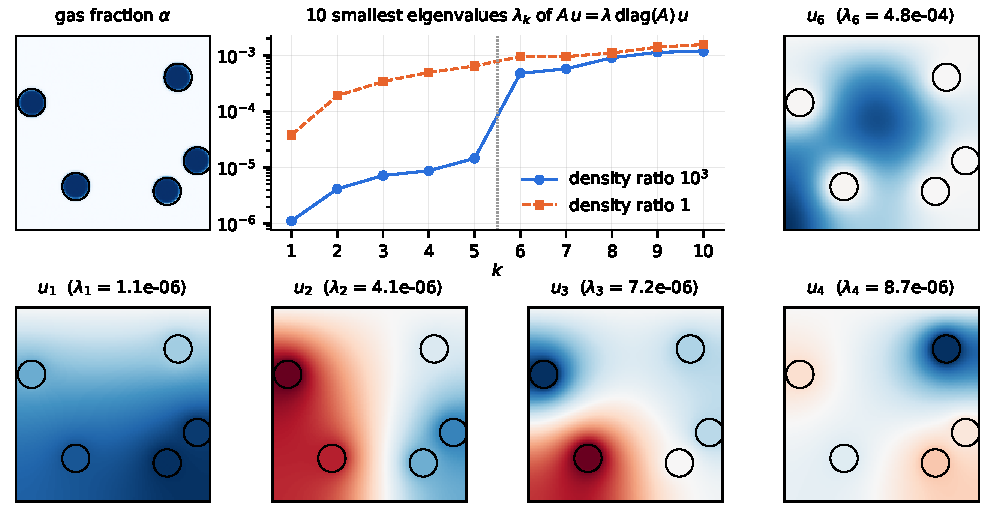
\includegraphics[width=\textwidth]{fig/bubble_modes.pdf}
  \caption{Near-kernel modes of the pressure matrix of a bubbly flow (2D, $128^2$ cells, five bubbles,
  density ratio $10^3$, $p=0$ on the top side). Top: gas fraction, the ten smallest eigenvalues of
  $Au=\lambda\,\mathrm{diag}(A)\,u$ with density ratio $10^3$ and $1$, and the sixth eigenvector, the first one
  above the gap. Bottom: the first four eigenvectors, nearly constant inside every bubble (black contours:
  $\alpha=0.5$). Matrices written by \texttt{matgen bubbles2d}, eigenpairs computed with SciPy (\texttt{fig/bubble\_modes.py}).}
  \label{fig:modes}
\end{figure}

\subsection{Overlapping Schwarz preconditioners}\label{sec:schwarz}

The notation follows~\cite{AlDaas2023,Dolean2015}. The unknowns $\{1,\dots,n\}$ are partitioned into $N$
non-overlapping sets $\Omega_{I,i}$ by a graph partitioner applied to $\mathcal{G}(A+A^\top)$. Each set is
extended by the nodes at distance one, $\Omega_{\Gamma,i}$, to obtain the overlapping subdomain
$\Omega_i = [\Omega_{I,i},\Omega_{\Gamma,i}]$ of size $n_i$. With the restriction $R_i = I_n(\Omega_i,:)$,
the local matrix $A_{ii}=R_iAR_i^\top$ and a partition of unity, i.e. non-negative diagonal matrices $D_i$
with $\sum_i R_i^\top D_i R_i = I_n$, the additive and restricted additive Schwarz preconditioners are
\begin{equation}\label{eq:onelevel}
  M^{-1}_{\mathrm{ASM}} = \sum_{i=1}^{N} R_i^\top A_{ii}^{-1} R_i , \qquad
  M^{-1}_{\mathrm{RAS}} = \sum_{i=1}^{N} R_i^\top D_i A_{ii}^{-1} R_i .
\end{equation}
Both exchange information only between neighbouring subdomains, so the number of iterations grows with
the number of subdomains, and a global correction is required~\cite[Ch.~4]{Dolean2015}. Given
$R_0\in\R^{n_0\times n}$ whose rows span a coarse space of dimension $n_0\ll n$ and $A_{00}=R_0AR_0^\top$,
the two-level preconditioners with additive and deflated coarse correction are
\begin{align}
  M^{-1}_{\star,\mathrm{additive}} &= R_0^\top A_{00}^{-1} R_0 + M^{-1}_{\star}, \label{eq:additive}\\
  M^{-1}_{\star,\mathrm{deflated}} &= R_0^\top A_{00}^{-1} R_0 + M^{-1}_{\star}\left(I - A R_0^\top A_{00}^{-1} R_0\right),
  \label{eq:deflated}
\end{align}
with $\star\in\{\mathrm{ASM},\mathrm{RAS}\}$. As in the experiments of~\cite{AlDaas2023}, the default
used in this work is RAS with the deflated correction.

\subsection{An algebraic spectral coarse space}\label{sec:coarse}

The coarse space of~\cite{AlDaas2023} is built from a local splitting of $A$ obtained by lumping. With the
local ordering $[\Omega_{I,i},\Omega_{\Gamma,i},\Omega^c_i]$, let $s_i$ be the vector of the absolute row
sums of the block $A(\Omega_{\Gamma,i},\Omega^c_i)$, i.e.\ of the couplings of the overlap nodes with the
outside of the subdomain. The local block splitting matrix is
\begin{equation}\label{eq:splitting}
  \At_{ii} = \begin{pmatrix} A_{I,i} & A_{I\Gamma,i}\\ A_{\Gamma I,i} & A_{\Gamma,i}-\mathrm{diag}(s_i)\end{pmatrix},
\end{equation}
which differs from $A_{ii}$ only on the diagonal of the overlap block and is therefore computed in $O(n_i)$
operations once the overlap rows are known. If $A$ is symmetric positive definite and diagonally dominant,
$\At_{ii}$ is a local positive semi-definite splitting of $A$~\cite[Lemma~3.2]{AlDaas2023}. The local
generalized eigenproblem is
\begin{equation}\label{eq:geneig}
  \Pi_i D_i A_{ii} D_i \Pi_i\,u = \lambda\,\At_{ii}\,u ,
\end{equation}
where $\Pi_i$ is the projection onto $\mathrm{range}(\At_{ii})$. With $L_i=\ker(D_iA_{ii}D_i)$ and
$K_i=\ker(\At_{ii})$, the local contribution $Z_i$ spans
\begin{equation}\label{eq:Zi}
  (L_i\cap K_i)^{\perp_{K_i}} \;\oplus\; \mathrm{span}\left\{u \;:\; \eqref{eq:geneig},\ |\lambda|\geq 1/\tau\right\},
\end{equation}
and the coarse space is spanned by the columns of $[R_1^\top D_1 Z_1,\dots,R_N^\top D_N Z_N]$. The first term
contains the eigenvectors of the infinite eigenvalues; it is not empty for floating subdomains, whose lumped
matrix has zero row sums and a non-trivial kernel. For symmetric positive definite and diagonally dominant
matrices the condition number of the additive two-level operator satisfies
\begin{equation}\label{eq:bound}
  \kappa_2\!\left(M^{-1}_{\mathrm{ASM,additive}}A\right) \leq (k_c+1)\left(2 + (2k_c+1)\frac{k_m}{\tau}\right),
\end{equation}
where $k_c$ is the number of colours needed to colour the subdomain graph and $k_m$ the maximum number of
subdomains sharing a row~\cite{AlDaas2023}: the bound does not depend on $N$ nor on the coefficients, and the
threshold $\tau$ trades the size of the coarse space for the condition number. In practice the number of
vectors per subdomain is also capped by a parameter \texttt{nev}. For non-symmetric matrices the same
construction is used without theoretical guarantee.

\subsection{Krylov methods and stopping tests}\label{sec:krylov}

The preconditioner is applied on the right inside restarted GMRES(30)~\cite{Saad1986}, as in the reference
paper, or BiCGStab~\cite{VanDerVorst1992}, the method of the \texttt{PBiCGStab} solver of OpenFOAM. Right
preconditioning keeps the stopping test on the unpreconditioned residual. Two tests are available: the
2-norm test $\|b-Ax\|_2\leq \mathrm{rtol}\,\|b\|_2$ of the paper, and the normalised residual of the
OpenFOAM solvers, $\sum|b-Ax|/F$ with
$F=\sum|Ax_0-\bar{x}A\mathbf{1}|+\sum|b-\bar{x}A\mathbf{1}|$ and $\bar{x}$ the mean of the initial guess,
with the \texttt{relTol} (relative) and \texttt{tolerance} (absolute) semantics of OpenFOAM. The second test is
what makes the comparison with GAMG fair: both codes stop at the same accuracy in the same norm.

% =============================================================================================
\section{Software architecture}\label{sec:architecture}
% =============================================================================================

\subsection{Requirements and design principles}

The architecture follows from the target use, a preconditioner that a CFD code could call at every
pressure solve:
\begin{itemize}
\item \textbf{Distributed by construction.} One MPI process owns one subdomain. After the decomposition no
  process holds global data: every global operation is a reduction, a neighbour exchange, or the assembly
  of the coarse matrix.
\item \textbf{The interface of a CFD code.} The only input of the preconditioner is the set of rows owned by
  a process, with global column indices and contiguous ownership ranges. This is exactly what an OpenFOAM
  processor has: the \texttt{lduMatrix} of its cells, the coefficients of its processor patches and a
  \texttt{globalIndex}.
\item \textbf{Algorithms and backends selected at run time.} Local and coarse direct solvers, approximate
  local solvers, Krylov methods and reuse policies are chosen from the command line, so that the same binary
  serves all campaigns; optional libraries are selected at compile time.
\item \textbf{Testable against sequential references.} Every distributed component has a test that compares
  it with a reference computed from the global matrix on one process.
\item \textbf{Measurable.} Every phase is timed by a scoped timer and reported as min/avg/max over the
  processes; every job records the sources and the environment it ran with.
\end{itemize}

\subsection{Code organization}

The library is split into six modules, each with its own directory under \texttt{include/} and
\texttt{src/} and its own namespace, and each component with a header and a source file.
\Cref{tab:modules} lists them and \cref{fig:modules} shows their dependencies. The structure is layered:
a module only depends on the modules below it, and the drivers are the only code that sees all of them.

\begin{table}[t]
  \centering\small
  \caption{Modules of the library (namespace \texttt{schwarz2lvl::<ns>}) and lines of code (headers + sources,
  comments included).}\label{tab:modules}
  \begin{tabularx}{\textwidth}{@{}l l X r@{}}
    \toprule
    Module & \texttt{ns} & Main classes & Lines\\
    \midrule
    \texttt{core} & \texttt{core} & scalar and index types, \texttt{SolverConfig} (command line), \texttt{LocalSystem}, MPI helpers & 694\\
    \texttt{partition} & \texttt{part} & \texttt{CsrMatrix}, \texttt{MatrixMarketIO}, \texttt{GraphPartitioner} (METIS), \texttt{DomainDecomposer}, \texttt{Subdomain} & 1509\\
    \texttt{linalg} & \texttt{linalg} & \texttt{HaloExchange}, \texttt{DistributedMatrix}, \texttt{LocalSolver} and its backends, AMG approximate inverse & 1304\\
    \texttt{preconditioner} & \texttt{prec} & \texttt{Preconditioner}, \texttt{OneLevelSchwarz}, \texttt{LocalEigensolver}, \texttt{CoarseSpace}, \texttt{CoarseSolver}, \texttt{TwoLevelSchwarz}, \texttt{ReusePolicy} & 2702\\
    \texttt{solver} & \texttt{solv} & \texttt{KrylovSolver}, \texttt{Gmres}, \texttt{BiCgStab}, \texttt{runTimeLoop} & 927\\
    \texttt{utils} & \texttt{utils} & \texttt{MatrixGenerator}, \texttt{BubbleField}, \texttt{TimerRegistry}, \texttt{Log} & 843\\
    \midrule
    drivers & - & \texttt{schwarz2lvl} (solver), \texttt{matgen} (test matrices) & 262\\
    tests & - & 9 MPI test programs, about 500 checks & 2680\\
    \bottomrule
  \end{tabularx}
\end{table}

\begin{figure}[t]
\centering
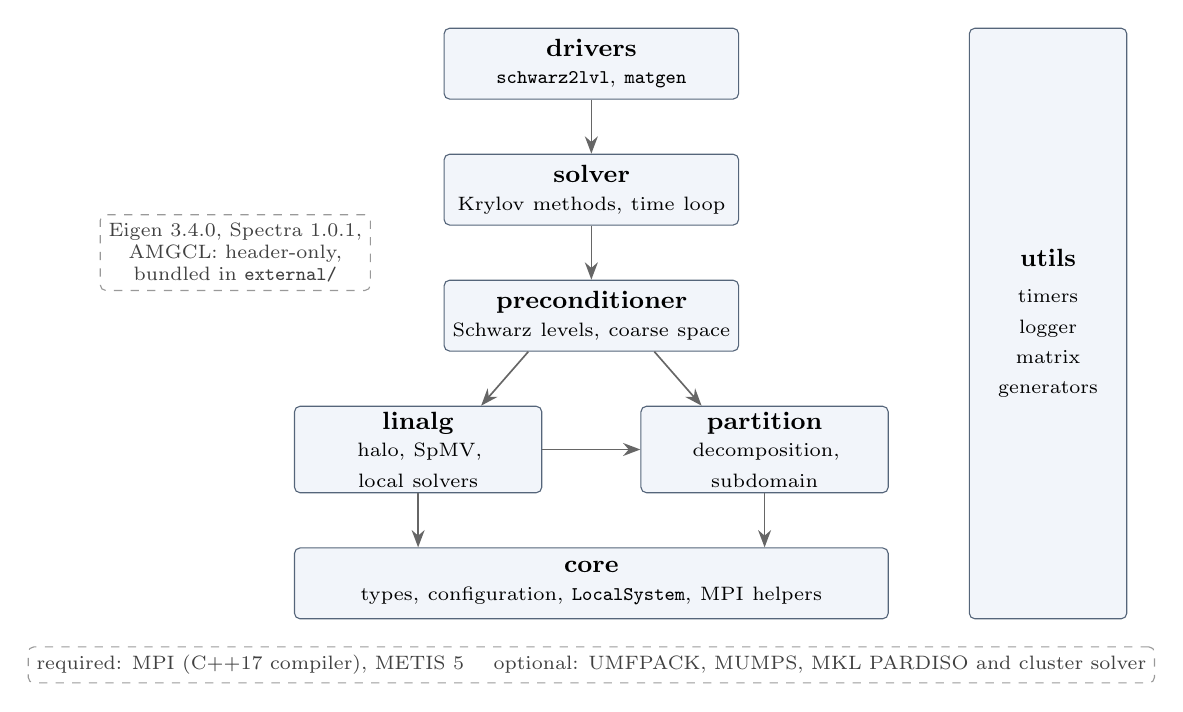
\begin{tikzpicture}[x=1mm,y=1mm,
  mod/.style={draw=boxedge,fill=boxfill,rounded corners=2pt,minimum height=9mm,text width=#1,
              align=center,font=\small,inner sep=2pt},
  mod/.default=36mm,
  ext/.style={draw=black!40,dashed,rounded corners=2pt,align=center,font=\scriptsize,text=black!75,inner sep=3pt},
  dep/.style={-{Stealth[length=2.2mm]},draw=black!60,line width=0.6pt}]
  \node[mod] (drv)  at (0,0)    {\textbf{drivers}\\[-1pt]\scriptsize\texttt{schwarz2lvl}, \texttt{matgen}};
  \node[mod] (solv) at (0,-16)  {\textbf{solver}\\[-1pt]\scriptsize Krylov methods, time loop};
  \node[mod] (prec) at (0,-32)  {\textbf{preconditioner}\\[-1pt]\scriptsize Schwarz levels, coarse space};
  \node[mod=30mm] (lin)  at (-22,-49) {\textbf{linalg}\\[-1pt]\scriptsize halo, SpMV, local solvers};
  \node[mod=30mm] (part) at (22,-49)  {\textbf{partition}\\[-1pt]\scriptsize decomposition, subdomain};
  \node[mod=74mm] (core) at (0,-66) {\textbf{core}\\[-1pt]\scriptsize types, configuration, \texttt{LocalSystem}, MPI helpers};
  \node[draw=boxedge,fill=boxfill,rounded corners=2pt,font=\small,align=center,
        minimum width=20mm,minimum height=75mm,inner sep=2pt] (utils) at (58,-33)
        {\textbf{utils}\\[2pt]\scriptsize timers\\ \scriptsize logger\\ \scriptsize matrix\\ \scriptsize generators};
  \draw[dep] (drv) -- (solv);
  \draw[dep] (solv) -- (prec);
  \draw[dep] ($(prec.south)+(-8,0)$) -- ($(lin.north)+(8,0)$);
  \draw[dep] ($(prec.south)+(8,0)$) -- ($(part.north)+(-8,0)$);
  \draw[dep] (lin) -- (part);
  \draw[dep] (lin.south) -- (lin.south |- core.north);
  \draw[dep] (part.south) -- (part.south |- core.north);
  \node[ext,anchor=east] (hdr) at (-28,-24) {Eigen 3.4.0, Spectra 1.0.1,\\ AMGCL: header-only,\\ bundled in \texttt{external/}};
  \node[ext,anchor=north] (libs) at (0,-74) {required: MPI (C++17 compiler), METIS 5 \quad
     optional: UMFPACK, MUMPS, MKL PARDISO and cluster solver};
\end{tikzpicture}
\caption{Module dependencies (an arrow reads ``uses''). \texttt{linalg} depends on \texttt{partition} only
through the \texttt{Subdomain} wrapped by \texttt{DistributedMatrix}. \texttt{utils} is cross-cutting: every
module uses its timers and logger, and the decomposition calls its matrix generators.}
\label{fig:modules}
\end{figure}

\subsection{Data distribution and communication}\label{sec:distribution}

\paragraph{Decomposition.} \texttt{DomainDecomposer} reproduces the \texttt{decomposePar} step of OpenFOAM:
rank~0 reads a Matrix Market file or runs a built-in generator, partitions $\mathcal{G}(A+A^\top)$ with
METIS~\cite{Karypis1998}, renumbers the unknowns so that process $p$ owns the contiguous range
$[o_p,o_{p+1})$, and sends to each process only its rows. For systems with several unknowns per cell the
graph is compressed by cells, so that the unknowns of a cell are never split. The result is a
\texttt{LocalSystem}, the only interface between the decomposition and the preconditioner:
\begin{lstlisting}
struct LocalSystem {
    MPI_Comm comm;                       // communicator of the decomposition
    GlobalIndex n_global;                // global number of unknowns
    std::vector<GlobalIndex> ownership;  // rank p owns [ownership[p], ownership[p+1])
    std::vector<GlobalIndex> row_ptr, col; // owned rows in CSR, global column indices
    std::vector<Scalar> val, rhs;        // values and owned right-hand side
    int block_size; bool symmetric;
};
\end{lstlisting}
Global indices are 64-bit and local ones 32-bit, so that large problems do not inflate the memory of the
local matrices.

\paragraph{Overlap and halo.} \texttt{Subdomain} builds everything a process knows about its overlapping
subdomain, collectively but without global data. The overlap $\Omega_{\Gamma,i}$ consists of the
off-process columns of the owned rows ($A$ part) and of the remote rows that have a column in
$\Omega_{I,i}$ ($A^\top$ part); the latter are discovered with one \texttt{MPI\_Alltoall} of counts and one
\texttt{MPI\_Alltoallv}, which makes the neighbour relation symmetric. The owners then send the full rows of
the ghost unknowns, the only extra matrix data the method needs, and the local matrices $A_{ii}$ (column
major, to be factorized) and $A(\Omega_{I,i},\Omega_i)$ (row major, for the products) are assembled; the
lumping sums $s_i$ of~\eqref{eq:splitting} are accumulated while the ghost rows are received.
The local numbering places the owned unknowns first, in global order, followed by the ghosts sorted by
global index (\cref{fig:layout}). Since ownership ranges are contiguous, the ghosts owned by one neighbour
form a contiguous block, which messages fill directly without unpacking.

\begin{figure}[t]
\centering
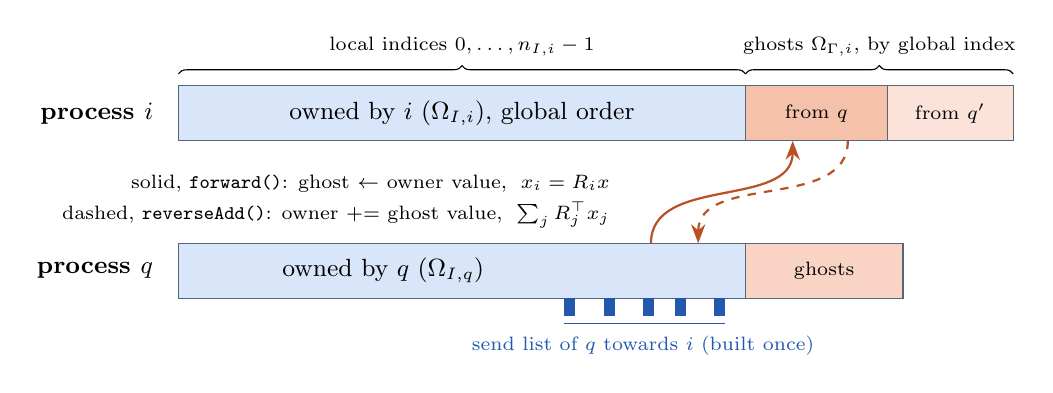
\begin{tikzpicture}[x=1mm,y=1mm]
  % process i
  \fill[schwarz!18] (0,10) rectangle (72,17);
  \fill[gamg!40] (72,10) rectangle (90,17);
  \fill[gamg!18] (90,10) rectangle (106,17);
  \draw[boxedge] (0,10) rectangle (106,17);
  \draw[boxedge] (72,10) -- (72,17) (90,10) -- (90,17);
  \node[font=\small] at (36,13.5) {owned by $i$ ($\Omega_{I,i}$), global order};
  \node[font=\scriptsize] at (81,13.5) {from $q$};
  \node[font=\scriptsize] at (98,13.5) {from $q'$};
  \node[anchor=east,font=\small\bfseries] at (-2,13.5) {process $i$};
  \draw[decorate,decoration={brace,amplitude=3pt}] (0,18.5) -- (72,18.5)
       node[midway,above=3pt,font=\scriptsize] {local indices $0,\dots,n_{I,i}-1$};
  \draw[decorate,decoration={brace,amplitude=3pt}] (72,18.5) -- (106,18.5)
       node[midway,above=3pt,font=\scriptsize] {ghosts $\Omega_{\Gamma,i}$, by global index};
  % process q
  \fill[schwarz!18] (0,-10) rectangle (72,-3);
  \fill[gamg!28] (72,-10) rectangle (92,-3);
  \draw[boxedge] (0,-10) rectangle (92,-3);
  \draw[boxedge] (72,-10) -- (72,-3);
  \node[font=\small] at (26,-6.5) {owned by $q$ ($\Omega_{I,q}$)};
  \node[font=\scriptsize] at (82,-6.5) {ghosts};
  \node[anchor=east,font=\small\bfseries] at (-2,-6.5) {process $q$};
  % send list of q towards i
  \foreach \x in {49,54,59,63,68} \fill[schwarz!80!black] (\x,-10) rectangle ++(1.4,-2.2);
  \draw[schwarz!80!black] (49,-13.2) -- (69.4,-13.2);
  \node[anchor=north,font=\scriptsize,schwarz!80!black] at (59,-13.6) {send list of $q$ towards $i$ (built once)};
  % the two operations
  \draw[-{Stealth[length=2.4mm]},line width=0.8pt,gamg!80!black] (60,-3) to[out=90,in=-90] (78,10);
  \draw[-{Stealth[length=2.4mm]},line width=0.8pt,dashed,gamg!80!black] (85,10) to[out=-90,in=90] (66,-3);
  \node[anchor=east,font=\scriptsize] at (56,4.6) {solid, \texttt{forward()}: ghost $\leftarrow$ owner value, \;$x_i = R_i x$};
  \node[anchor=east,font=\scriptsize] at (56,0.6) {dashed, \texttt{reverseAdd()}: owner $\mathrel{+}=$ ghost value, \;$\sum_j R_j^\top x_j$};
\end{tikzpicture}
\caption{Local numbering of the vectors and the two operations of \texttt{HaloExchange}. On process $i$ the
owned unknowns come first and the ghosts follow, sorted by global index: with contiguous ownership ranges the
ghosts owned by one neighbour form a contiguous block, which a message fills in place. The entries a process
sends to each neighbour (its send lists) are computed once, when the subdomain is built; both operations use
non-blocking point-to-point messages between neighbours only.}
\label{fig:layout}
\end{figure}

\paragraph{Communication patterns.} \texttt{HaloExchange} implements the two operators of the method with
non-blocking point-to-point messages to the neighbours only: \texttt{forward()} realizes $R_i$ (every ghost
receives the owner's value) and \texttt{reverseAdd()} realizes $\sum_j R_j^\top$ (ghost values are sent back
and added to the owned ones). A templated \texttt{exchange<T>()} sends irregular data (ghost rows, sparse rows
of the coarse basis) with a size handshake. \texttt{DistributedMatrix} computes $y=Ax$ as one
\texttt{forward()} followed by a local product with the owned rows, the scheme of \texttt{Amul} in
OpenFOAM. Distributed vectors store only the owned entries, so inner products are local products followed by
one \texttt{MPI\_Allreduce}. With the Boolean partition of unity ($D_i=1$ on $\Omega_{I,i}$, $0$ on the
ghosts), RAS needs no reverse communication and the restriction and prolongation of the coarse correction
are purely local: one application of~\eqref{eq:deflated} costs two \texttt{forward()} exchanges (local solve
and extra product) and the collectives of the coarse solve.

\subsection{Class design of the preconditioner}\label{sec:classes}

\Cref{fig:classes} shows the main classes. The design combines dynamic polymorphism, where a choice is made
at run time and the cost of a virtual call is negligible against the work it triggers (a sparse solve or a
coarse correction), with templates, where variants differ only in types known at compile time (precision,
Eigen solver, MPI datatype).

\begin{figure}[t]
\centering
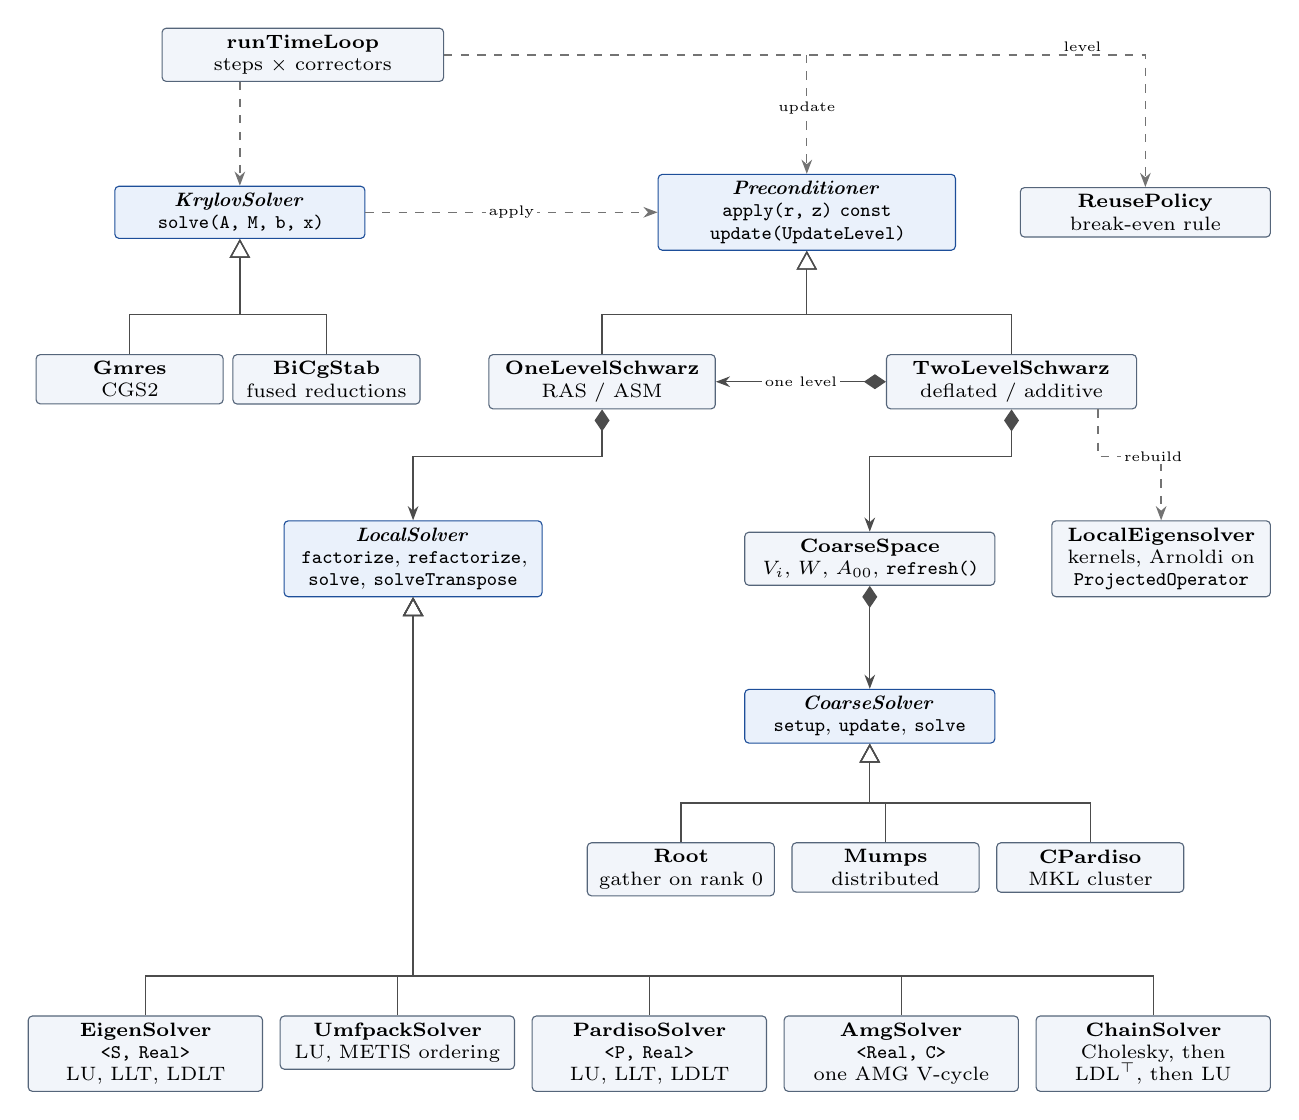
\begin{tikzpicture}[x=1mm,y=1mm,
  cls/.style={draw=boxedge,fill=boxfill,rounded corners=1.5pt,align=center,font=\scriptsize,
              inner sep=2.5pt,text width=#1},
  cls/.default=26mm,
  abs/.style={cls=#1,fill=schwarz!10,draw=schwarz!70!black},
  abs/.default=26mm,
  inh/.style={-{Triangle[open,length=2.4mm,width=2.6mm]},draw=black!70,line width=0.5pt},
  comp/.style={{Diamond[length=2.8mm,width=1.9mm]}-{Stealth[length=1.8mm]},draw=black!70,line width=0.5pt},
  use/.style={-{Stealth[length=1.8mm]},draw=black!55,dashed,line width=0.5pt},
  lab/.style={font=\tiny,fill=white,inner sep=1pt}]
  % row 1: time loop
  \node[cls=34mm] (TL) at (-44,0) {\textbf{runTimeLoop}\\ steps $\times$ correctors};
  % row 2: interfaces used by the loop
  \node[abs=30mm] (K) at (-52,-20) {\textbf{\textit{KrylovSolver}}\\ \texttt{solve(A, M, b, x)}};
  \node[abs=36mm] (P) at (20,-20) {\textbf{\textit{Preconditioner}}\\ \texttt{apply(r, z) const}\\ \texttt{update(UpdateLevel)}};
  \node[cls=30mm] (RP) at (63,-20) {\textbf{ReusePolicy}\\ break-even rule};
  % row 3
  \node[cls=22mm,anchor=north] (G) at (-66,-38) {\textbf{Gmres}\\ CGS2};
  \node[cls=22mm,anchor=north] (B) at (-41,-38) {\textbf{BiCgStab}\\ fused reductions};
  \node[cls=27mm,anchor=north] (O) at (-6,-38) {\textbf{OneLevelSchwarz}\\ RAS / ASM};
  \node[cls=30mm,anchor=north] (T) at (46,-38) {\textbf{TwoLevelSchwarz}\\ deflated / additive};
  % row 4
  \node[abs=31mm] (L) at (-30,-64) {\textbf{\textit{LocalSolver}}\\ \texttt{factorize}, \texttt{refactorize},\\ \texttt{solve}, \texttt{solveTranspose}};
  \node[cls=30mm] (CS) at (28,-64) {\textbf{CoarseSpace}\\ $V_i$, $W$, $A_{00}$, \texttt{refresh()}};
  \node[cls=26mm] (LE) at (65,-64) {\textbf{LocalEigensolver}\\ kernels, Arnoldi on\\ \texttt{ProjectedOperator}};
  % row 5-6: coarse solvers
  \node[abs=30mm] (C) at (28,-84) {\textbf{\textit{CoarseSolver}}\\ \texttt{setup}, \texttt{update}, \texttt{solve}};
  \node[cls=22mm,anchor=north] (Ro) at (4,-100) {\textbf{Root}\\ gather on rank 0};
  \node[cls=22mm,anchor=north] (Mu) at (30,-100) {\textbf{Mumps}\\ distributed};
  \node[cls=22mm,anchor=north] (Cp) at (56,-100) {\textbf{CPardiso}\\ MKL cluster};
  % row 7: local solver backends
  \node[cls=28mm,anchor=north] (E)  at (-64,-122) {\textbf{EigenSolver}\\ \texttt{<S, Real>}\\ LU, LLT, LDLT};
  \node[cls=28mm,anchor=north] (U)  at (-32,-122) {\textbf{UmfpackSolver}\\ LU, METIS ordering};
  \node[cls=28mm,anchor=north] (Pa) at (0,-122)   {\textbf{PardisoSolver}\\ \texttt{<P, Real>}\\ LU, LLT, LDLT};
  \node[cls=28mm,anchor=north] (A)  at (32,-122)  {\textbf{AmgSolver}\\ \texttt{<Real, C>}\\ one AMG V-cycle};
  \node[cls=28mm,anchor=north] (Ch) at (64,-122)  {\textbf{ChainSolver}\\ Cholesky, then\\ LDL$^\top$, then LU};
  % uses from the time loop
  \draw[use] (TL.south -| K.north) -- (K.north);
  \draw[use] (TL.east) -- (RP.north |- TL.east) -- (RP.north);
  \draw[use] (TL.east -| P.north) -- (P.north) node[lab,pos=0.45] {update};
  \node[lab,anchor=south] at ($(RP.north |- TL.east)+(-8,0)$) {level};
  \draw[use] (K.east) -- (P.west) node[lab,midway] {apply};
  % inheritance
  \foreach \n in {G,B} \draw[inh] (\n.north) -- ++(0,5) -| (K.south);
  \foreach \n in {O,T} \draw[inh] (\n.north) -- ++(0,5) -| (P.south);
  \foreach \n in {Ro,Mu,Cp} \draw[inh] (\n.north) -- ++(0,5) -| (C.south);
  \foreach \n in {E,U,Pa,A,Ch} \draw[inh] (\n.north) -- ++(0,5) -| (L.south);
  % composition and use
  \draw[comp] (T.west) -- (O.east) node[lab,midway] {one level};
  \draw[comp] (O.south) -- ++(0,-6) -| (L.north);
  \draw[comp] (T.south) -- ++(0,-6) -| (CS.north);
  \draw[use] ($(T.south)+(11,0)$) -- ++(0,-6) -| (LE.north);
  \node[lab] at ($(T.south)+(18,-6)$) {rebuild};
  \draw[comp] (CS.south) -- (C.north);
\end{tikzpicture}
\caption{Main classes of the preconditioner and the solvers (italic: abstract interfaces). Open triangles
denote inheritance, diamonds ownership through \texttt{std::unique\_ptr}, dashed arrows use. Concrete objects
are created by factories (\texttt{makeLocalSolver}, \texttt{makeCoarseSolver}, \texttt{makeKrylovSolver}) from
the configuration; the template parameters select the Eigen or PARDISO solver type, the precision of the
factors (\texttt{double} or \texttt{float}) and the AMG coarsening. \texttt{LocalEigensolver} and
\texttt{Root} factorize their matrices through a \texttt{ChainSolver}. The data classes of
\cref{sec:distribution} (\texttt{Subdomain}, \texttt{HaloExchange}, \texttt{DistributedMatrix}), which all
of them use, are omitted.}
\label{fig:classes}
\end{figure}

\paragraph{Preconditioner.} The abstract class \texttt{Preconditioner} exposes the application
$z=M^{-1}r$ on owned vectors and an \texttt{update(UpdateLevel)} method that brings the preconditioner up to
date with new matrix values (\cref{sec:reuse}). \texttt{OneLevelSchwarz} implements~\eqref{eq:onelevel}
with one \texttt{LocalSolver} for $A_{ii}$. \texttt{TwoLevelSchwarz} is composed of a \texttt{OneLevelSchwarz},
the result of the \texttt{LocalEigensolver} and a \texttt{CoarseSpace}, which owns the \texttt{CoarseSolver}
of $A_{00}$; its \texttt{apply()} is a direct transcription of~\eqref{eq:additive} - \eqref{eq:deflated}
(deflated variant, timers omitted):

\noindent\begin{minipage}{\linewidth}
\begin{lstlisting}[language=C++,
                   directivestyle={\color{black}},
                   emph={apply,char,double,float,unsigned},
                   emphstyle={\color{schwarz}}
                  ]
coarse_->apply(r, x0_);          // x0 = R0^T A00^{-1} R0 r
A_.apply(x0_, w_);               // deflated variant: one extra product
w_ = r - w_;
one_->apply(w_, z1_);            // M_RAS^{-1} (r - A x0)
z = x0_ + z1_;
\end{lstlisting}
\end{minipage}

\paragraph{Local solvers.} \texttt{LocalSolver} is a strategy interface for sequential sparse solvers:
\texttt{factorize()}, \texttt{refactorize()} (numerical factorization reusing the symbolic analysis, with a
fallback to a full factorization), multi right-hand-side \texttt{solve()} and \texttt{solveTranspose()}. The
backends are the Eigen solvers~\cite{Eigen} (SparseLU, SimplicialLLT, SimplicialLDLT), UMFPACK~\cite{Davis2004}
called directly on the compressed arrays of the Eigen matrix, MKL PARDISO~\cite{MKL}, and one V-cycle of
AMGCL~\cite{Demidov2019} as an approximate inverse. Precision is a template parameter: with
\texttt{float} the matrix is converted once, the right-hand side is rounded and the solution converted back,
and \texttt{if constexpr} removes every conversion in the \texttt{double} instantiation. \texttt{ChainSolver}
composes solvers of decreasing requirements (Cholesky, then LDL$^\top$, then LU): it tries each candidate
until one factorizes, and later refactorizations start from the one that worked. A symmetric factorization
is requested only if the matrix is known to be symmetric, since it reads only one triangle. The factory
\texttt{makeLocalSolver(spec)} builds the right object from a small specification (backend, request,
symmetry, precision, approximation).

\paragraph{Coarse solvers.} \texttt{CoarseSolver} receives the coarse matrix as distributed triplets whose
duplicates must be summed. \texttt{RootCoarseSolver} gathers them on rank~0 and factorizes with a
\texttt{LocalSolver} chain; \texttt{MumpsCoarseSolver} passes them to MUMPS~\cite{Amestoy2001} as a
distributed assembled matrix, optionally on a subset of leader processes; \texttt{CPardisoCoarseSolver} uses
the cluster version of PARDISO with distributed rows, and checks every distributed Cholesky factorization with
a probe solve, because with several processes MKL does not report a matrix that is not positive definite. The
choice between a distributed solver and rank~0 is made collectively from $n_0$: for small coarse problems the
fixed cost of the collectives of a distributed solve dominates.

\paragraph{Krylov solvers.} \texttt{KrylovSolver} has two implementations. \texttt{Gmres} orthogonalizes
with classical Gram - Schmidt applied twice (CGS2), so that the $j$ inner products of a pass need a single
reduction (three reductions per iteration instead of $j+1$ with modified Gram--Schmidt), and accepts
convergence only if the true residual, recomputed explicitly, is within $10\%$ of the tolerance. With the 
OpenFOAM test it reconstructs $\sum|r_j|$ from the Krylov basis and the Givens rotations at every iteration. 
\texttt{BiCgStab} follows the algorithm of OpenFOAM's \texttt{PBiCGStab} (right preconditioning, stopping test 
at the half step) with the reductions fused into four per step instead of six. In both, an iteration is an 
application of the preconditioner, so that iteration counts and costs compare directly.

\subsection{The local eigensolver}\label{sec:eigensolver}

$\At_{ii}$ is singular for every floating subdomain, so it can never be factorized as it is, and the
infinite eigenvalues of~\eqref{eq:geneig} must be separated from the finite ones. \texttt{LocalEigensolver}
does this explicitly:
\begin{enumerate}
\item factorize $\At_{ii}+\sigma I$ with $\sigma=10^{-13}\|\At_{ii}\|$, a regularization at the level of
  round-off (Cholesky chain for symmetric matrices);
\item detect the kernel $K_i$ by block inverse iteration with that factorization (three multi right-hand-side
  solves, block enlarged while all probes lie in the kernel), followed by an SVD of $\At_{ii}Y$; for
  non-symmetric matrices the left kernel is computed in the same way with transposed solves;
\item compute $(L_i\cap K_i)^{\perp_{K_i}}$ exactly from the SVD of $B_iQ$, $B_i=D_iA_{ii}D_i$, instead of
  relying on eigenvalues ``close to $\varepsilon^{-1}$'';
\item compute the largest finite eigenvalues with the implicitly restarted Arnoldi method of
  Spectra~\cite{Spectra}, applied matrix-free to $T=\Pi_K(\At_{ii}+\sigma I)^{-1}\Pi_R B_i\Pi_K$, where
  $\Pi_K$ and $\Pi_R$ project out the right and left kernels: each application costs one SpMV and one pair of
  triangular solves.
\end{enumerate}
The operator $T$ is a small adapter class, \texttt{ProjectedOperator}, with the interface that Spectra
expects (\texttt{rows()}, \texttt{cols()}, \texttt{perform\_op()}); it also counts and times its
applications. Only eigenvalues with $|\lambda|\geq1/\tau$ are kept, so instead of computing \texttt{nev}
eigenpairs at once the solver starts with $k=32$ and enlarges $k$ until the smallest computed modulus falls
below $1/\tau$: the selected vectors are the same, but the cost follows the number of selected vectors. A
complex pair contributes the real and imaginary parts of its eigenvector, which span the same real invariant
subspace, so the whole code works in real arithmetic. Subdomains with fewer than 400 unknowns use a dense
path (SVD and full eigendecomposition), which is also the reference of the tests.

\subsection{Coarse assembly without global data}\label{sec:coarseassembly}

\texttt{CoarseSpace} orthonormalizes $D_iZ_i$ with a column-pivoted QR, which keeps the span, drops dependent
vectors and gives a better conditioned $A_{00}$. Process $i$ owns the $m_i$ coarse unknowns generated by its
basis $V_i$; their global numbering needs one \texttt{MPI\_Allgather}. The coarse matrix
$A_{00}=R_0AR_0^\top$ with $R_0^\top=[R_1^\top V_1,\dots,R_N^\top V_N]$ is assembled from local products only:
\begin{equation}\label{eq:a00}
  A_{00} = \sum_{i=1}^{N} W(\Omega_{I,i},:)^\top\, A(\Omega_{I,i},\Omega_i)\, W(\Omega_i,:),
\end{equation}
where $W=R_0^\top$ restricted to $\Omega_i$ is obtained with one forward exchange of sparse rows. Each process
contributes the triplets of its term, and the coarse solver sums them. Since $W$ depends only on the basis, it
is kept: when the values of $A$ change but the basis does not, \texttt{refresh()} recomputes~\eqref{eq:a00}
with two local products and the coarse solver only refactorizes numerically.

\subsection{Setup reuse along a sequence of matrices}\label{sec:reuse}

In a CFD time loop the sparsity pattern of the pressure matrix never changes, its values change slightly at
every step and not at all between the correctors of one step. Creating a new preconditioner at every solve
throws away work that depends only on the pattern. The setup is therefore split by what each part depends on
(\cref{tab:reuse}), and \texttt{update()} redoes only what is needed at one of three levels.

\begin{table}[t]
\centering\small
\caption{What each part of the setup depends on and what each update level recomputes. The basis $V_i$ is
kept by a refactorization: it was computed for the matrix of the last rebuild.}\label{tab:reuse}
\setlength{\tabcolsep}{4pt}
\begin{tabularx}{\textwidth}{@{}l X l ccc@{}}
\toprule
Depends on & Data & Code & Reuse & Refactorize & Rebuild\\
\midrule
graph of $A$ & overlap, halo, patterns, $D_i$ & \texttt{Subdomain} (constructor) & kept & kept & kept\\
values of $A$ & $A_{ii}$, $A(\Omega_I,\Omega_i)$, $s_i$ & \texttt{Subdomain::updateValues} & kept & refilled & refilled\\
pattern of $A_{ii}$ & symbolic factorization of $A_{ii}$ & \texttt{LocalSolver} & kept & kept & redone\\
values of $A$ & numerical factorization of $A_{ii}$ & \texttt{LocalSolver} & kept & redone & redone\\
values of $A$ & $\At_{ii}$, eigenproblems, $V_i$, $W$ & \texttt{LocalEigensolver} & kept & \textbf{kept (old)} & redone\\
$A$ and $V$ & $A_{00}$ and its factorization & \texttt{CoarseSpace::refresh} & kept & redone & redone\\
\bottomrule
\end{tabularx}
\end{table}

\texttt{Subdomain::updateValues()} computes once, at construction, the position in the value arrays of the
local matrices of every owned and received coefficient; afterwards a change of values costs one halo
exchange of the ghost-row values (no indices) and an indexed copy. A \texttt{Refactorize} keeps the coarse
basis of the last rebuild but recomputes $A_{00}$ with the current matrix, so the preconditioner remains a
valid preconditioner of the new matrix; only its coarse space is tuned to an older one, and the iterations
grow as the bubbles move away.

When to rebuild is decided by \texttt{ReusePolicy} with a break-even rule. Let $q_{\mathrm{ref}}$ be the
number of iterations per decade of residual reduction of the first solve after the last rebuild. Every later
solve with $k$ iterations and $d$ decades wastes $(k-q_{\mathrm{ref}}\,d)\,t_{\mathrm{it}}$ seconds because of
the old basis; a rebuild is requested when the time wasted since the last rebuild reaches the extra cost of
a rebuild over a refactorization, both measured during the run. This is the classical rent-or-buy decision:
it adapts by itself to the machine, the subdomain size and the contrast, with no threshold to tune. Two
details made it robust on the cluster: the costs are the lower medians of all the measured rebuilds and
refactorizations, so that a single stalled factorization does not freeze the rebuilds, and with warm starts or
different tolerances per corrector each corrector index keeps its own $q_{\mathrm{ref}}$. Since all decisions
are local floating-point computations, \texttt{update()} first agrees on the maximum requested level over all
processes: a process refactorizing while another rebuilds would deadlock in the collectives of the coarse
solver.

\subsection{C++ techniques}\label{sec:cpp}

\begin{itemize}
\item \textbf{Ownership and RAII.} Components are owned through \texttt{std::unique\_ptr} and created by
  factories; resources of external libraries are released in destructors (UMFPACK symbolic and numeric
  objects, MUMPS instances, MPI communicators created with \texttt{MPI\_Comm\_split}). \texttt{ScopedTimer}
  measures the lifetime of a scope and accumulates it in a registry, so timing a phase is a one-line
  declaration that cannot be left unbalanced by an early return or an exception.
\item \textbf{Templates where types vary.} The trait \texttt{mpiType<T>()} maps C++ types to MPI datatypes,
  so that generic helpers (\texttt{allreduceSum<T>}, \texttt{HaloExchange::exchange<T>}) are type safe; the
  solver backends are class templates over the Eigen or PARDISO solver type and over the precision.
\item \textbf{Collective error handling.} An exception thrown on one process while the others enter a
  collective would hang the job. Failures that can occur on a subset of processes (a factorization, a local
  eigensolve, the decomposition on rank~0) are therefore turned into a status that is reduced over all
  processes before any of them throws, so every process reports the error.
\item \textbf{Configuration.} \texttt{SolverConfig} parses the command line through a table that maps each
  option name to a lambda setting the corresponding field, followed by a \texttt{validate()} step: adding an
  option is one line, and invalid combinations are rejected before any MPI work starts.
\item \textbf{Documentation.} Every class and function is documented with Doxygen comments that refer to the
  equations of the paper (\texttt{make doc}).
\end{itemize}

\subsection{Performance engineering}\label{sec:perfeng}

Several implementation details changed the cost by large factors without changing the preconditioner; each
was identified from the timers and verified to leave $n_0$ and the iteration counts unchanged:
\begin{itemize}
\item \textbf{No iterative refinement in the direct solvers.} The Eigen interface of PARDISO enables two
  refinement steps per solve by default, which made every local solve $3$--$3.7\times$ slower; inside a
  preconditioner and an eigensolver the backward error of the factorization is sufficient. UMFPACK runs with
  METIS ordering and no refinement as well (on a $36^3$ convection--diffusion matrix: $31\%$ fewer nonzeros in
  the factors and a $2.1\times$ faster numerical factorization).
\item \textbf{Block operations in the eigensolver.} The kernel detection solves all probe vectors in one
  multi right-hand-side call per inverse-iteration step.
\item \textbf{Small coarse problems on one process} (\texttt{--coarse-root-below}): below $n_0=10^4$ the
  gather to rank~0 is cheaper than a distributed solve on G100.
\item \textbf{Warm-up of the direct solver.} In the first run of two G100 jobs the factorizations of the
  eigensolver took 14--19\,s over the whole run on every process, while a complete rebuild took 1.5\,s; the
  initial setup then entered the reuse policy as the cost of a rebuild and delayed the first rebuild by several
  steps. The cause was not pinned down. Every run now factorizes a small Laplacian with the local backend
  before the time loop, untimed, which keeps any such start-up cost out of the measurements and out of the
  decisions of the policy (initial setup / median rebuild $=0.98$--$1.03$ in all later runs).
\item \textbf{Fewer reductions in the Krylov methods}: CGS2 in GMRES and fused reductions in BiCGStab
  (\cref{sec:classes}).
\end{itemize}

\subsection{Build, tests and reproducibility}\label{sec:build}

The code is built with a Makefile. The only mandatory external dependencies are an MPI C++17 compiler and
METIS; Eigen~3.4.0, Spectra~1.0.1 and AMGCL are header-only and bundled. UMFPACK and MUMPS are enabled
automatically when their headers are found, and MKL is enabled with a switch; without them the code is
complete, with the Eigen solvers for the local matrices and the coarse matrix on rank~0.

\Cref{tab:tests} lists the nine test programs. They build sequential references from the global matrix,
broadcast to every process, and compare the distributed objects with them; every check is combined over the
processes, so a failure on one rank fails the test. \texttt{make check} runs every test with 1, 2 and 4
processes. A build with AddressSanitizer and UndefinedBehaviorSanitizer ran the whole suite without any
memory or undefined-behaviour report.

\begin{table}[t]
\centering\small
\caption{Test programs and number of checks with 4 processes in the default build (UMFPACK and MUMPS
enabled).}\label{tab:tests}
\begin{tabularx}{\textwidth}{@{}l X r@{}}
\toprule
Test & What is compared with a sequential reference & Checks\\
\midrule
\texttt{test\_subdomain} & overlap, halo, $A_{ii}$, lumping sums, partition of unity, SpMV; symmetry detection & 32\\
\texttt{test\_preconditioner} & sparse vs dense eigensolver (kernels, eigenvalues, residuals of~\eqref{eq:geneig}); RAS/ASM $\times$ deflated/additive against a reference assembled on one process; GMRES & 192\\
\texttt{test\_reuse} & refactorization and refresh vs fresh setup on time-dependent matrices; reuse policy; time loop & 108\\
\texttt{test\_factorization} & Cholesky/LDL$^\top$/LU chains, single precision, every coarse solver of the build & 97\\
\texttt{test\_inexact} & AMG V-cycle as local solver: linearity, determinism, two-level GMRES with the same coarse space & 22\\
\texttt{test\_stopping}, \texttt{test\_bicgstab} & OpenFOAM stopping test, GMRES and BiCGStab, iteration budget & 26\\
\texttt{test\_warmstart}, \texttt{test\_bubbles} & p\_rgh right-hand side, absolute tolerances, warm start; bubble field shared with OpenFOAM & 21\\
\bottomrule
\end{tabularx}
\end{table}

Every campaign on G100 is one SLURM job script that builds its own copy of the binaries, runs the unit tests
on the compute nodes, and records the hash of the sources and the loaded modules next to the results; a
Python script turns the raw logs into the report and the plots of the campaign. All the numbers of
\cref{sec:results} can be regenerated from the files committed in the repository.

% =============================================================================================
\section{Results}\label{sec:results}
% =============================================================================================

\subsection{Platform and methodology}

All runs were made on the thin nodes of CINECA Galileo100: two 24-core Intel Xeon processors (Cascade Lake)
per node, 384\,GB of memory, InfiniBand interconnect; one MPI process per core and one subdomain per process.
On G100 the code was compiled with the OpenFOAM-10 toolchain (Intel MPI 2021), METIS 5.1.0 and MKL
2023.2.0, PARDISO for the local matrices and the MKL cluster solver for large coarse problems. The cost of a
solve includes the setup and the updates amortized over the sequence (initial setup + updates + Krylov
iterations, divided by the number of solves), measured between two barriers. Where the network produced
timing bursts, costs were also compared with median times; the conclusions were the same.

\subsection{Reproduction of the reference paper}\label{sec:paper}

The experiments of Section~4 of~\cite{AlDaas2023} were repeated on 240 processes (instead of 256), with
METIS instead of ParMETIS, PARDISO instead of MUMPS for the local factorizations and Spectra instead of
SLEPc; the convection--diffusion problem~(4.1) of the paper was discretized with upwind finite volumes instead
of SUPG finite elements. \Cref{tab:table1} compares the SuiteSparse matrices of Table~1. The paper states
$\tau=0.6$, but its row for G3\_circuit coincides with the point $\tau=0.9$ of its own Figure~2; the
comparison is therefore made at $\tau=0.9$, where the coarse space per subdomain is within $15\%$ of the paper
on 8 of 10 matrices.

\begin{table}[t]
\centering\small
\caption{Table~1 of~\cite{AlDaas2023} (GMRES(30), $\mathrm{rtol}=10^{-8}$, \texttt{nev}$=300$) against this
implementation at $\tau=0.9$, 240 processes. n.c.: not converged in 200 iterations.}\label{tab:table1}
\begin{tabular}{@{}lrrrrr@{}}
\toprule
& \multicolumn{2}{c}{Paper} & \multicolumn{2}{c}{This work} & One-level RAS\\
\cmidrule(lr){2-3}\cmidrule(lr){4-5}
Matrix & iterations & $n_0/N$ & iterations & $n_0/N$ & iterations\\
\midrule
finan512    & 6  & 10  & 6  & 22  & 6\\
nxp1        & 20 & 77  & 29 & 95  & n.c.\\
CoupCons3D  & 20 & 113 & 21 & 98  & 23\\
tmt\_unsym  & 6  & 129 & 5  & 128 & n.c.\\
ecology2    & 6  & 133 & 5  & 130 & n.c.\\
thermal2    & 26 & 157 & 5  & 139 & n.c.\\
atmosmodj   & 7  & 298 & 14 & 286 & 79\\
G3\_circuit & 8  & 279 & 7  & 279 & n.c.\\
Transport   & 9  & 300 & 8  & 300 & n.c.\\
memchip     & 36 & 226 & 8  & 224 & 44\\
\bottomrule
\end{tabular}
\end{table}

The iteration counts agree within one iteration on six matrices; nxp1 and atmosmodj need more iterations
with a coarse space of similar size, thermal2 and memchip fewer. For non-symmetric matrices the count also
depends on the partition and on the random right-hand side, which differ between the two codes. Wherever
one-level RAS does not converge, the two-level method does. \Cref{fig:g3} reproduces the effect of $\tau$ on
G3\_circuit: $n_0$ follows the paper within $15\%$ except at $\tau=0.6$ ($-26\%$), and the iterations are
$9$--$29\%$ lower. In strong scaling (Figure~4 of the paper, three-dimensional problem (4.1) with
$8\times10^6$ unknowns) the iterations stay bounded, $16\to12$ from 30 to 240 processes, and the time
decreases from 187\,s to 16.8\,s: the superlinear speedup comes from the factorizations and the local
eigensolves, whose cost grows faster than linearly with the subdomain size. For the convection--diffusion
problem of Table~2 the trends of the paper are reproduced; the coarse space is smaller than in the paper
($0.5$--$0.6\times$ in 2D, $0.2\times$ in 3D), consistently with the smaller stencils of the finite volume
discretization, which reduce the lumping, and in 3D with $\nu\leq10^{-3}$ this costs iterations.

\begin{figure}[t]
  \centering
  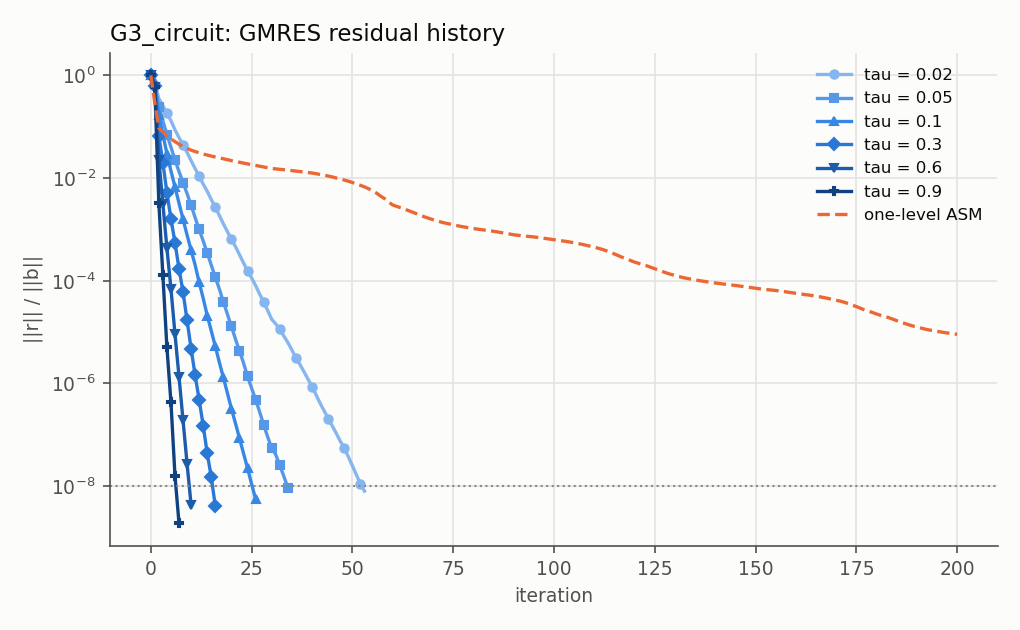
\includegraphics[width=0.66\textwidth]{fig/paper_g3circuit_tau.png}
  \caption{G3\_circuit, 240 processes: residual history of GMRES(30) with the two-level preconditioner for the
  values of $\tau$ of Figure~2 of~\cite{AlDaas2023}, and one-level ASM.}
  \label{fig:g3}
\end{figure}

\subsection{Optimizations for sequences of systems}\label{sec:phases}

The following phases adapted the method to a time loop on the bubbly-flow problem of \cref{sec:problem}
(150 bubbles of radius $0.04$, density ratio $10^3$, three correctors per step, every solve from zero with a
new random right-hand side, GMRES(30) to $\mathrm{rtol}=10^{-8}$). \Cref{tab:phases} summarizes them; on
the $192^3$ mesh ($7.1$ million unknowns, 240 processes) they reduced the cost of a solve from $16.0$\,s with a
new preconditioner at every solve to about $0.5$\,s.

\begin{table}[t]
\centering\small
\caption{Optimization phases on G100: cost per solve, setup and updates included. Last column: before
$\to$ after the phase on the $192^3$ mesh with 240 processes, each phase measured in its own job. Details in the
\texttt{RESULTS.md} files of \texttt{test/reuse}, \texttt{test/cholesky}, \texttt{test/p5} and
\texttt{test/p7}.}\label{tab:phases}
\begin{tabularx}{\textwidth}{@{}l X X r@{}}
\toprule
Phase & Change & Outcome (all measured cases) & $192^3$ [s/solve]\\
\midrule
P1 & setup reuse: refactorizations, rebuild at break-even (\cref{sec:reuse}) & $5.7$--$7.4\times$ cheaper than a new preconditioner at every solve & $16.0\to2.62$\\
P2 & Cholesky instead of LU for $A_{ii}$, $\At_{ii}+\sigma I$, $A_{00}$ & $-10\%$ to $-18\%$; identical iterations & $2.40\to2.15$\\
P5 & small coarse space: cap \texttt{nev}$=8$ instead of $\tau$ alone & $-52\%$ to $-80\%$ (rebuilds $4$--$6\times$ cheaper) & $2.09\to0.99$\\
P7 & one AMG V-cycle (smoothed aggregation, Gauss--Seidel) instead of the exact factors of $A_{ii}$ & $-26\%$ to $-56\%$ & $1.00\to0.51$\\
\bottomrule
\end{tabularx}
\end{table}

\Cref{fig:reuse} shows the effect of setup reuse. Without a coarse space, RAS needs about 800 iterations
per solve. With the reuse policy the two-level preconditioner is refactorized at every step and rebuilt
when the aging basis has wasted as much time as a rebuild costs: the iterations follow a saw-tooth from 12 to
31--39, and the total cost is the same as that of never rebuilding (\texttt{refactor}), whose iterations grow
from 12 to 47 in 12 steps and then settle around 30. At the lower density ratio $10$ the basis barely ages and
the policy rebuilds only twice in 60 steps. Phase P2 changed only the cost of the factorizations: the iteration
sequences are identical. Phase P5 showed that a coarse space of 8 vectors per subdomain is enough at this
density ratio: every coarse operation becomes cheaper and Arnoldi computes fewer eigenpairs, so a rebuild is
$4$--$6\times$ cheaper and the policy rebuilds more often, which keeps the average iterations unchanged. In P7,
one V-cycle of smoothed-aggregation AMG behaves as an exact local solve on these matrices: the first solve after
a rebuild needs the same iterations at $192^3$ ($24.7$ against $24.5$) and $3.7$ more at $256^3$, while the
local solves are $3.4$--$4.4\times$ cheaper, since the exact 3D factors have $20$--$35$ times the nonzeros of
$A_{ii}$ and a V-cycle reads about $1.5\,\mathrm{nnz}(A_{ii})$ a few times. Ideas that did not pay off were
measured and removed: incomplete Cholesky local solvers (not spectrally equivalent: $2.4$--$8.7\times$ the
iterations), other AMG smoothers, reusing the AMG hierarchy across refactorizations, single-precision factors
as a default, a larger coarse space at the practical tolerance, warm-started eigenvectors and the reuse of the
factorization of $\At_{ii}$ between rebuilds.

\begin{figure}[t]
  \centering
  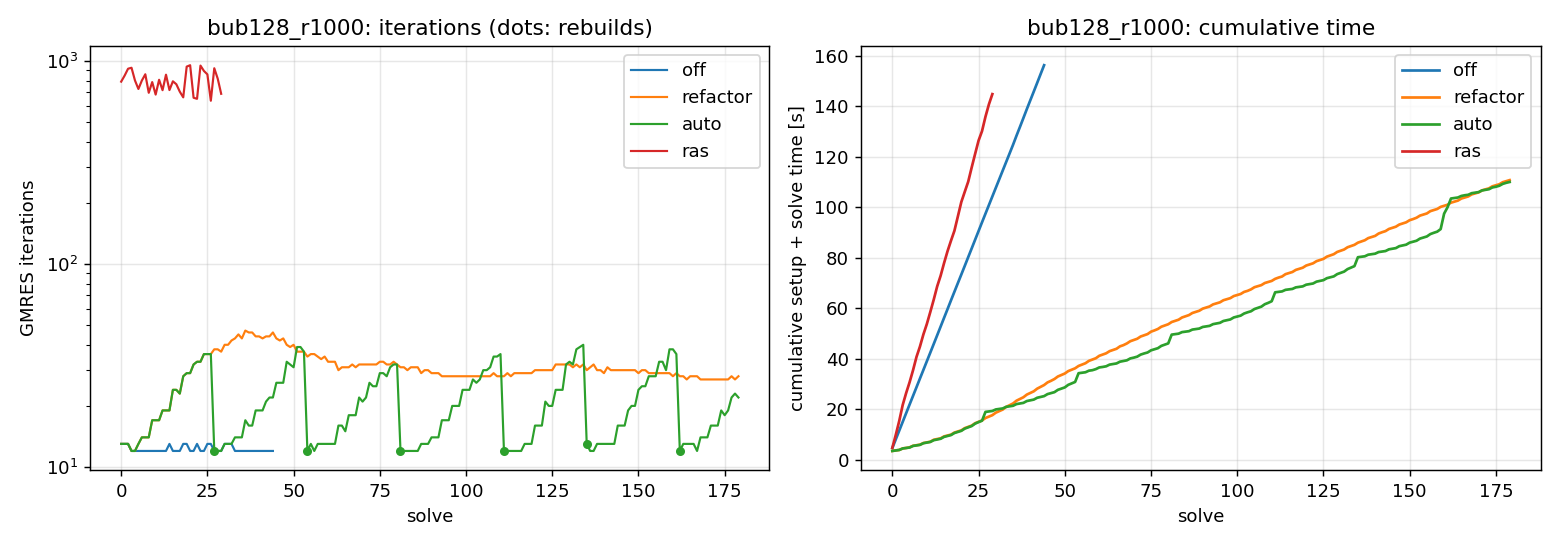
\includegraphics[width=\textwidth]{fig/reuse_bub128.png}
  \caption{Setup reuse on the bubbles problem ($128^3$, density ratio $10^3$, 240 processes, GMRES to
  $10^{-8}$). \texttt{off}: new setup before every solve; \texttt{refactor}: numerical refactorizations, basis
  never rebuilt; \texttt{auto}: break-even rule (dots: rebuilds); \texttt{ras}: one-level RAS.}
  \label{fig:reuse}
\end{figure}

\subsection{Comparison with the GAMG solver of OpenFOAM}\label{sec:gamg}

\paragraph{Set-up.} A small OpenFOAM-10 application, \texttt{bubblyPressureFoam}, assembles
\eqref{eq:pressure} on a uniform mesh with the bubble field of the generator (a header-only class shared by the
two codes) and solves it with the OpenFOAM solvers. Before every campaign the matrix and the right-hand side
written by OpenFOAM are compared with those of the generator: they agree to $3.6\times10^{-15}$ relative to the
largest entry, and the jobs stop otherwise. This check found a real discrepancy: compiled with the Intel
compiler and aggressive optimization, the bubble field of the OpenFOAM application placed 2 of 150 bubbles
elsewhere; the field is now compiled with the same compiler as \texttt{schwarz2lvl} and linked through a C
interface. GAMG runs with the OpenFOAM defaults (\texttt{faceAreaPair} agglomeration); the DIC smoother was the
fastest OpenFOAM variant in a first comparison against Gauss--Seidel, \texttt{algebraicPair} agglomeration and
GAMG-preconditioned CG. The two-level preconditioner uses the settings of phases P5 and P7 (\texttt{--tau 0.3
--nev 8}, AMG local solves, reuse \texttt{auto}). Meshes of $192^3$, $256^3$ and $320^3$ cells
($7.1$, $16.8$ and $32.8$ million unknowns) were run on 240, 336 and 432 processes.

\paragraph{Every solve from zero.} To $\|r\|_2/\|b\|_2\leq10^{-8}$ on 240 processes the two-level method
needs 51 iterations on average at both $192^3$ and $256^3$, while GAMG needs 139 and 271 V-cycles: it is
$2.0\times$ and $4.3\times$ faster per solve. At the tolerance used by OpenFOAM in a time step
(\texttt{relTol} $10^{-2}$ of the normalised residual) the gain is smaller but holds on all nine
configurations (\cref{tab:scaling}): $1.8$--$2.7\times$.

\begin{table}[t]
\centering\small
\caption{Cost per solve [s] at \texttt{relTol} $10^{-2}$, every solve from zero, 16 steps $\times$ 3
correctors (S: two-level Schwarz with GMRES(30); G: GAMG with the DIC smoother) and ratio G/S.}\label{tab:scaling}
\begin{tabular}{@{}lccc@{}}
\toprule
& 240 processes & 336 processes & 432 processes\\
\midrule
$192^3$ & S 0.316 \,·\, G 0.567 \,·\, \textbf{1.79}$\times$ & S 0.258 \,·\, G 0.570 \,·\, \textbf{2.21}$\times$ & S 0.206 \,·\, G 0.563 \,·\, \textbf{2.73}$\times$\\
$256^3$ & S 0.986 \,·\, G 1.99\phantom{0} \,·\, \textbf{2.02}$\times$ & S 0.724 \,·\, G 1.65\phantom{0} \,·\, \textbf{2.28}$\times$ & S 0.573 \,·\, G 1.48\phantom{0} \,·\, \textbf{2.59}$\times$\\
$320^3$ & S 2.38\phantom{0} \,·\, G 4.74\phantom{0} \,·\, \textbf{1.99}$\times$ & S 1.80\phantom{0} \,·\, G 3.39\phantom{0} \,·\, \textbf{1.88}$\times$ & S 1.12\phantom{0} \,·\, G 2.74\phantom{0} \,·\, \textbf{2.44}$\times$\\
\bottomrule
\end{tabular}
\end{table}

\begin{figure}[t]
  \centering
  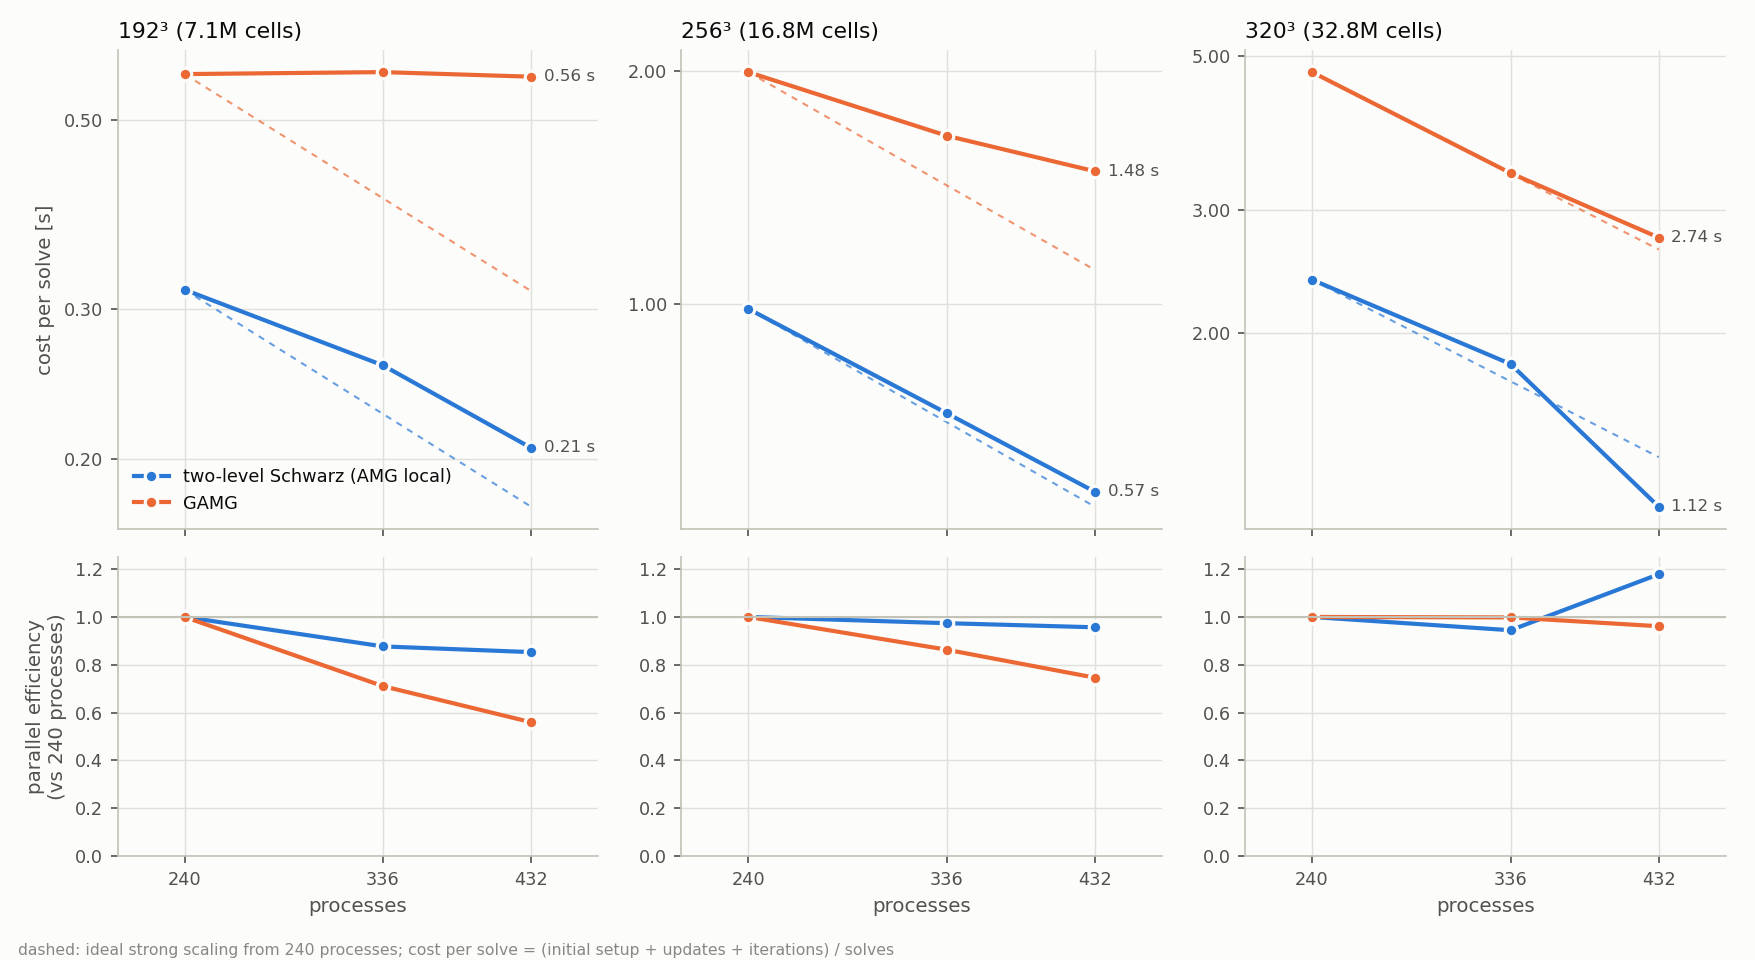
\includegraphics[width=\textwidth]{fig/gamg_scaling_strong.png}
  \caption{Strong scaling at \texttt{relTol} $10^{-2}$: cost per solve (top; dashed: ideal from 240
  processes) and parallel efficiency relative to 240 processes (bottom).}
  \label{fig:strong}
\end{figure}

\begin{figure}[t]
  \centering
  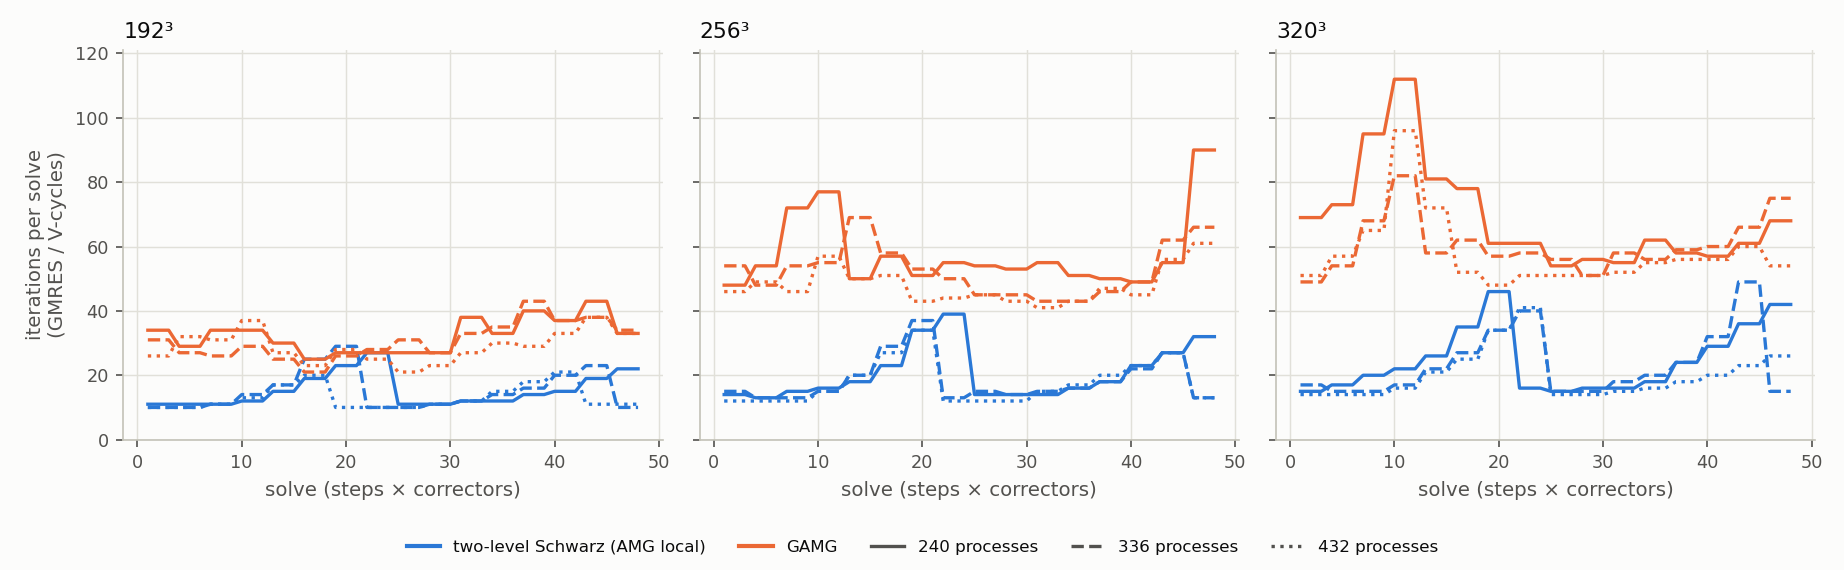
\includegraphics[width=\textwidth]{fig/gamg_scaling_iterations.png}
  \caption{Iterations of the two-level Schwarz preconditioner (GMRES) and V-cycles of GAMG for every solve of
  the time loop. The saw-tooth of the Schwarz iterations is the aging of the coarse space between two rebuilds.}
  \label{fig:iterations}
\end{figure}

One iteration of the two-level method costs about as much as one V-cycle of GAMG at 240 processes
($34.8$ against $34.5$\,ms at $256^3$, $68.9$ against $68.8$\,ms at $320^3$): the whole gain is in the number
of iterations, $2.0$--$2.9\times$ fewer. From $192^3$ to $320^3$ GAMG goes from 32 to 69 V-cycles per solve,
while the Schwarz iterations right after a rebuild go from 11 to 15 (\cref{fig:iterations}). The two-level
method also scales better (\cref{fig:strong}): the parallel efficiency from 240 to 432 processes is
$0.85$/$0.96$/$1.18$ against $0.56$/$0.75$/$0.96$ for GAMG ($192^3$/$256^3$/$320^3$), and at $192^3$ GAMG does
not speed up at all because its V-cycle becomes slower on more processes. In the Schwarz cost, setup and
updates take about $30\%$, the local AMG V-cycles $21$--$33\%$, the coarse correction $11$--$29\%$ (growing
with the number of processes) and the Krylov method itself $17$--$27\%$, most of it in the orthogonalization and
the stopping test of GMRES.

\paragraph{Krylov method.} BiCGStab has a fixed amount of vector work per application of the preconditioner and
explicit residuals, which makes the OpenFOAM stopping test nearly free. With the same preconditioner it needs
$1.04$--$1.20\times$ the applications of GMRES, each $0.72$--$0.85\times$ as expensive, for a cost per solve of
$1.02$, $0.89$ and $0.82\times$ that of GMRES at $192^3$, $256^3$ and $320^3$ (\cref{fig:krylov}). Since it is
the algorithm of \texttt{PBiCGStab}, a port could use the existing OpenFOAM solver with the two-level Schwarz
as its preconditioner. Two further campaigns tuned the coarse space. A looser tolerance of the Arnoldi method
(\texttt{--eig-tol 1e-2 --eig-ncv 12}) needs 27--29 applications of the operator instead of 42 and reduces
the initial setup by $18\%$, with the same iterations after every rebuild: the bubble modes have large,
well separated eigenvalues and converge in a few steps, while resolving the cluster just above $1/\tau$ to high
accuracy adds cost and nothing to the preconditioner. A larger coarse space, 12 or 16 vectors per subdomain
instead of 8, reduced the iterations by $8$--$22\%$ but increased the cost per solve by $4$--$20\%$, because
the coarse correction and the setup grow with \texttt{nev}; the gain in iterations also vanishes on the finest
mesh, and the coarse space ages just as fast.
With BiCGStab, \texttt{nev}$=8$ and the looser Arnoldi, the setting used in the next campaign, the two-level
method is $2.0$, $2.6$ and $2.5\times$ faster than GAMG on 240 processes at $192^3$, $256^3$ and $320^3$.

\begin{figure}[t]
  \centering
  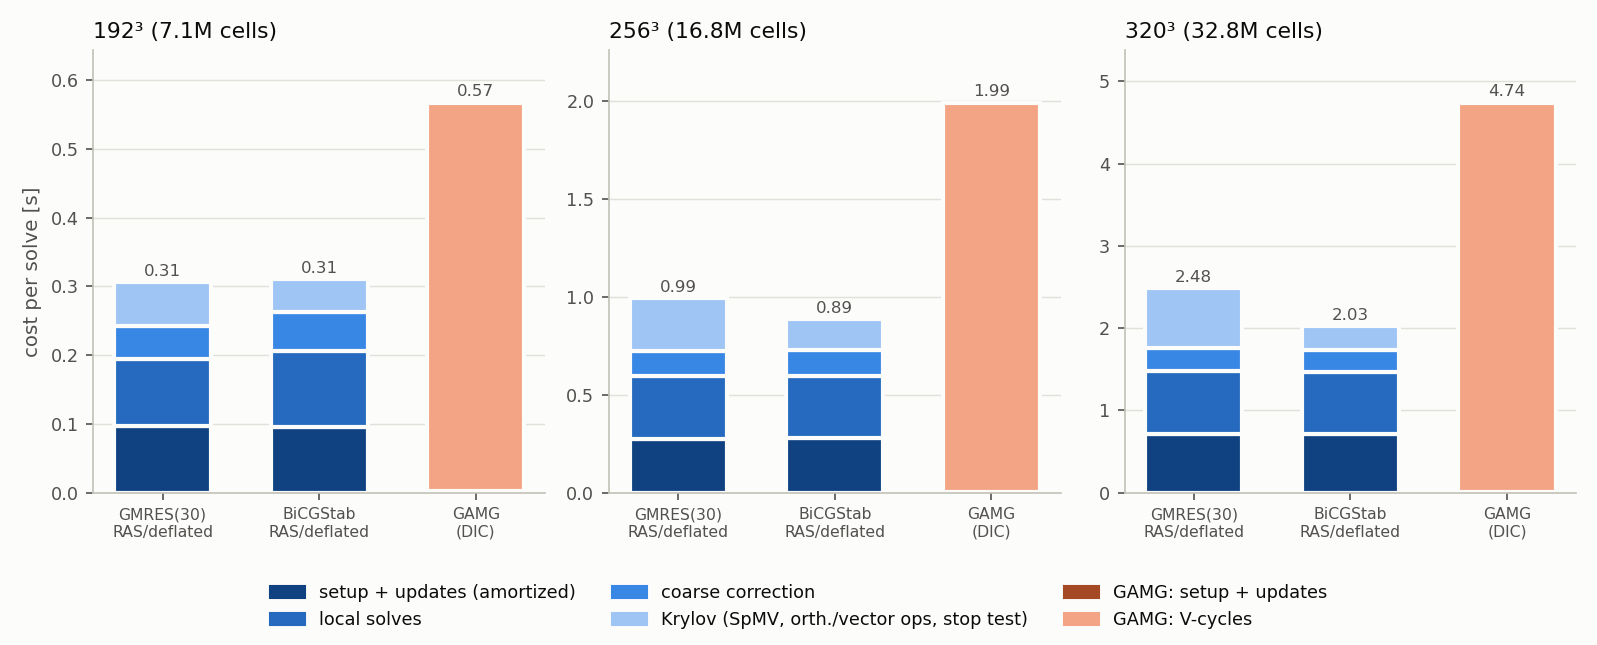
\includegraphics[width=\textwidth]{fig/gamg_krylov_cost.png}
  \caption{Cost per solve at 240 processes, \texttt{relTol} $10^{-2}$: two-level Schwarz with GMRES(30) and
  BiCGStab, split into setup and updates, local solves, coarse correction and Krylov work, and GAMG.}
  \label{fig:krylov}
\end{figure}

\paragraph{A PIMPLE-like time loop.} The comparisons above solve every system from zero with a right-hand
side constant on every bubble, which projects almost entirely on the near-kernel modes of \cref{fig:modes}.
An OpenFOAM time loop differs in three ways: the source of the $p_{rgh}$ equation of a volume-of-fluid
solver lives on the interfaces and sums to zero over every bubble, every solve starts from the previous
solution, and only the last corrector of a step is converged tightly. The last campaign reproduced these
conditions: right-hand side $-\nabla\cdot\phi_g$ of interFoam for the fluid at rest, warm starts, the first
two correctors to \texttt{relTol} $0.05$ (or tolerance $10^{-7}$), the last one to tolerance $10^{-7}$, the
settings of the \texttt{p\_rgh}/\texttt{p\_rghFinal} controls of the OpenFOAM tutorials. The two codes solve
the same sequence: the initial normalised residual of the first corrector of every step agrees between them
to $3\times10^{-5}$. A decision rule was written
before the run: a port is justified if the two-level method is at least about $1.5\times$ faster than the best
OpenFOAM variant at both process counts.

\begin{table}[t]
\centering\small
\caption{PIMPLE-like loop (24 steps $\times$ 3 correctors, warm start): cost per time step [s], all correctors,
setup and updates included, and average iterations of the last corrector (applications of the preconditioner /
V-cycles). Schwarz with BiCGStab, \texttt{nev}$=8$, AMG local solves; GAMG\_DIC is the fastest OpenFOAM
variant.}\label{tab:warm}
\begin{tabular}{@{}rrrrrrr@{}}
\toprule
& & \multicolumn{3}{c}{Cost per time step [s]} & & \multicolumn{1}{c}{Last corrector}\\
\cmidrule(lr){3-5}\cmidrule(lr){7-7}
Mesh & Proc. & Schwarz 2-level & RAS 1-level & GAMG\_DIC & GAMG/Schwarz & Schwarz / GAMG\\
\midrule
$192^3$ & 240 & 0.605 & 3.27 & 0.581 & \textbf{0.96}$\times$ & 22.5 / 35.2\\
$256^3$ & 240 & 1.68  & 11.2 & 1.97  & \textbf{1.17}$\times$ & 29.8 / 56.2\\
$320^3$ & 240 & 4.30  & 26.2 & 5.08  & \textbf{1.18}$\times$ & 38.4 / 71.9\\
$192^3$ & 432 & 0.358 & 1.90 & 0.647 & \textbf{1.81}$\times$ & 19.3 / 33.8\\
$256^3$ & 432 & 0.911 & 6.85 & 1.51  & \textbf{1.66}$\times$ & 24.0 / 53.0\\
$320^3$ & 432 & 2.06  & 15.2 & 2.79  & \textbf{1.35}$\times$ & 30.5 / 59.7\\
\bottomrule
\end{tabular}
\end{table}

\Cref{tab:warm} and \cref{fig:warm} summarize the result. The two-level method is faster than GAMG in five of
six configurations ($1.17$--$1.81\times$) and equal at $192^3$ on 240 processes. The gain now lives entirely
in the last corrector, where it is $2.0$--$4.1\times$; on the first two correctors, 1.3 decades from a good
initial guess, GAMG is $1.2$--$1.7\times$ cheaper, because little of the error lies in the bubble modes and
the coarse correction is paid for at every application without being needed. Setup and rebuilds are
$39$--$43\%$ of the Schwarz cost: the iterations became cheaper, the setup did not. The one-level RAS keeps up
on the first correctors but needs 420--700 applications on the last one, $2.9$--$5.7\times$ the cost of GAMG:
with $p$ prescribed only on the top face, the low-energy modes span the whole domain, and only the coarse
space makes the tight final tolerance affordable. By the rule written before the run, a port is not justified
as it stands: the threshold is reached only on 432 processes for the two smaller meshes.

\begin{figure}[t]
  \centering
  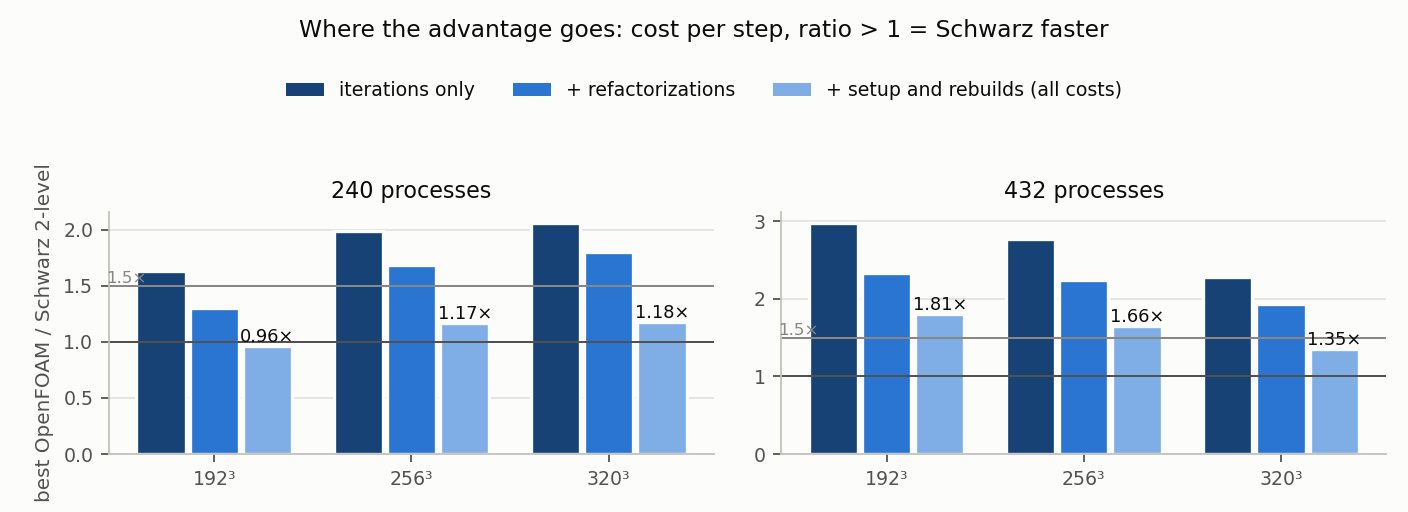
\includegraphics[width=\textwidth]{fig/gamg_warm_ratio.png}
  \caption{PIMPLE-like loop: ratio of the cost per time step of the best OpenFOAM variant to that of the
  two-level Schwarz preconditioner, built up phase by phase (iterations only; with refactorizations; with
  setup and rebuilds). Horizontal lines: parity and the $1.5\times$ threshold of the decision rule.}
  \label{fig:warm}
\end{figure}

\subsection{Interpretation}\label{sec:interpretation}

The measurements are consistent with the mechanism of \cref{sec:problem}. GAMG pairs cells by face area; on a
uniform mesh its aggregates ignore the interfaces and straddle them, so the modes that are nearly constant on
each bubble are left to the smoother, which propagates information by a few cells per sweep, while a bubble
spans 15 cells at $192^3$ and 26 at $320^3$: the number of V-cycles grows with the mesh. The local eigenproblems
of the two-level method select, in every subdomain, precisely the low-energy modes, whatever the shape of the
bubble pieces it contains, so the iterations grow only mildly. The price is that the coarse space follows the
bubbles: within 8--12 time steps (4--6 cells of rise) the iterations of the last corrector grow by a factor
$2.9$--$4.0$ and the basis must be rebuilt, at a cost that GAMG, whose agglomeration ignores the coefficients,
never pays. The PIMPLE-like campaign also shows that a right-hand side constant on the bubbles, solved from
zero, overstates the difficulty of the problem for GAMG: in a small local test $99\%$ of the energy of the
initial error lay in the ten lowest modes with that right-hand side, and less than $0.1\%$ with the $p_{rgh}$
source and a warm start.

% =============================================================================================
\section{Discussion and future work}\label{sec:discussion}
% =============================================================================================

\paragraph{Limitations of the study.} The comparison with GAMG covers one problem (a bubbly flow with density
ratio $10^3$) on uniform meshes, with OpenFOAM~10 while the target would be a more recent version, and different
decompositions in the two codes (scotch for OpenFOAM, METIS here). Each configuration of the last campaign was
run once; earlier campaigns showed a run-to-run spread of $\pm3$--$4\%$. The source term of a real flow also
contains the divergence of the predicted velocity, which is not confined to the interfaces. Finally, the
matrices of \texttt{schwarz2lvl} are generated on rank~0 and this time is not counted: it is a property of the
test harness (OpenFOAM assembles in parallel), but it makes a Schwarz job longer than a GAMG job in wall time.

\paragraph{Limitations of the implementation.} Real matrices only; one subdomain per MPI process; the global
matrix is read on rank~0 during the decomposition; local indices and the interfaces to the coarse solvers
(MUMPS, MKL with 32-bit integers) are limited to $2^{31}$ entries. For non-symmetric or indefinite matrices outside the class of~\cite{AlDaas2023} the coarse
space carries no guarantee.

\paragraph{Next steps.} The part of the cost left to reduce is keeping the coarse space up to date: rebuilds
and the aging between them account for most of the difference between the cold-start and the PIMPLE-like
results. The modes that age are those nearly constant on bubbles that have moved; a natural candidate is to
keep the eigenvectors of the last rebuild and add, at every step, indicator vectors of the gas regions of each
subdomain, computed from the current coefficients in $O(n_i)$ and assembled into $A_{00}$ at every
refactorization. A distributed generation of the matrix values would more than halve the core-hours of the Schwarz test runs. If the
preconditioner is ported to OpenFOAM, the natural form is an \texttt{lduMatrix::preconditioner} used by the
existing \texttt{PBiCGStab}, with the subdomain structure, the coarse space and the reuse policy stored in a
persistent object (e.g.\ a \texttt{MeshObject}, as GAMG stores its agglomeration), and \texttt{LocalSystem}
filled directly from the processor matrix.

% =============================================================================================
\section{Conclusions}\label{sec:conclusions}
% =============================================================================================

The algebraic two-level Schwarz preconditioner of Al~Daas, Jolivet and Rees was implemented in C++17/MPI as a
library whose only input is the set of rows owned by each process, the data an OpenFOAM processor has. The
implementation reproduces the experiments of the reference paper on 240 processes, and its distributed
components are verified against sequential references by about 500 automated checks.

On the pressure equation of a bubbly flow with density ratio $10^3$, the setup was adapted to sequences of
matrices with numerical refactorizations and a break-even rebuild rule, a small coarse space and AMG local
solves, which together reduced the cost of a solve about thirty times with respect to rebuilding the
preconditioner at every solve ($16.0\to0.51$\,s on $7.1$ million unknowns and 240 processes). On identical matrices of up to $32.8$ million unknowns the two-level method
is $1.8$--$2.7\times$ faster than the GAMG solver of OpenFOAM when every system is solved from zero to the
OpenFOAM tolerance, $2.0$--$4.3\times$ to $10^{-8}$, and it scales better. The gain is algorithmic: one iteration
costs as much as a V-cycle, but the spectral coarse space captures the near-kernel modes of the bubbles that
the geometric agglomeration of GAMG cannot represent. In a PIMPLE-like loop with warm starts the advantage
shrinks to $0.96$--$1.81\times$ per time step and is concentrated in the tightly converged last corrector, while
setup and rebuilds become $40\%$ of the cost. By the criterion fixed in advance, a port to OpenFOAM is not yet
justified; a coarse space that follows the bubbles at the cost of a refactorization is the step that could
change this conclusion.

\bibliographystyle{unsrtnat}
\bibliography{refs}

\end{document}
